\section{Teoria Relativistica dei Campi}
\subsection{Campi e trasformazioni dei campi}
Un campo è una regione nella quale ad ogni punto della varietà è associata una quantità di una determinata grandezza fisica. In particolare, la quantificazione è data da una legge rappresentabile secondo una certa funzione $f$. A seconda della natura della funzione, il campo può assumere la caratterizzazione di scalare, spinoriale, vettoriale o tensoriale.

Le teorie relativistiche di campo sono modelli teorici utilizzati nella fisica delle particelle. Ad ogni particella si associa un campo, in particolare vengono usati campi quantistici. Semplificando, la modellizzazione consiste nel vedere un campo come una collezione di infiniti oscillatori armonici, la quantizzazione del campo avviene nel considerare gli oscillatori armonici come quantistici. Ogni oscillatore armonico quantistico possiede uno stato fondamentale non triviale, se tutti gli oscillatori armonici sono nello stato fondamentale il campo viene detto \textit{vuoto}. Infatti, le particelle possono essere viste come eccitazioni quantizzate degli oscillatori rispetto allo stato fondamentale. Particelle con spin nullo sono descritte da campi scalari, un esempio è lo scalare di Higgs. I quarks e i leptoni, che hanno spin $\frac{1}{2}$, sono descritti da campi spinoriali. Le particelle di spin pari a uno sono descritti da campi quadrivettoriali, un esempio ne è il fotone. La caratterizzazione dei campi (quindi scalare, spinoriale e quatrivettoriale) è riferita alle trasformazioni di Lorenz, anzi più in generale al gruppo di Poincaré. Queste teorie non considerano la gravità, infatti sono utilizzabili in casi particolari nei quali la gravità è nulla o risulta essere trascurabile.

Consideriamo una trasformazione di Lorentz
\begin{equation}
  x^\mu\xrightarrow[\text{}]{\text{L}}x'^{\mu}=\Lambda\indices{^\mu_\nu} x^{\nu} 
\end{equation}
a sua volta il campo subisce una trasformazione del tipo:
\begin{equation}
  f(x^\mu)\xrightarrow[\text{$x^\mu\xrightarrow[\text{}]{\text{}}x'^{\mu}$}]{\text{L}}f'(x'^{\mu})
\end{equation}
quindi non vi è solo il cambio dell'argomento, bensì anche il campo stesso subisce una variazione.

Considerando una trasformazione infinitesima 
\begin{equation}
  x^\mu\xrightarrow[\text{}]{\text{L}}x'^{\mu}=x^{\mu} +\delta x^\mu
\end{equation}
possiamo quindi definire la \textit{variazione totale} del campo come:
\begin{equation}
\begin{aligned}
\delta f&=f'(x'^\mu)-f(x^\mu)=f'(x^\mu+\delta x^\mu)-f(x^\mu)=f'(x^\mu)+\delta x^\mu\partial_\mu f(x^\mu)-f(x^\mu)\\
&=f'(x^\mu)-f(x^\mu)+\delta x^\mu\partial_\mu f(x^\mu)=\delta_0 f +\delta x^\mu\partial_\mu f(x^\mu)
\end{aligned}
\end{equation}
ove il termine $f'(\delta x^\mu)=\delta x^\mu\partial_\mu f(x^\mu)$ è dato dal fatto che lavoriamo al primo ordine in $\delta x^\mu$, allora dobbiamo prendere $f'$ all'ordine zero, che è appunto $f$. Inoltre, $\delta_0 f$ è detta \textit{variazione funzionale}, mentre il termine $\delta x^\mu\partial_\mu f(x^\mu)$ è detto \textit{termine di trasporto}.

A questo punto consideriamo le trasformazioni di Poincaré, in particolare partiamo dalle traslazioni, quindi:
\begin{equation}
  x^\mu\xrightarrow[\text{}]{\text{P}}x'^{\mu}= x^{\mu} +a^\mu
\end{equation}
sotto traslazione non c'è variazione di un campo locale, ossia:
\begin{equation}
  f(x^\mu)\xrightarrow[\text{$x^\mu\xrightarrow[\text{}]{\text{}}x^{\mu} +a^\mu$}]{\text{T}}f'(x'^{\mu})=f(x^\mu)
\end{equation}
quindi la variazione totale sarà nulla
\begin{equation}
    \delta f=f'(x'^\mu)-f(x^\mu)=0
\end{equation}
quindi avremo che la variazione funzionale sarà pari al termine di trasporto cambiato di segno:
\begin{equation}
    \delta_0 f =-\delta x^\mu\partial_\mu f(x^\mu)=-\mathcal{E}^\mu \partial_\mu f=-i\mathcal{E}^\mu \hat{P}_\mu f
\end{equation}
ove nel penultimo passaggio abbiamo usato il fatto che $\delta x^\mu=x'^\mu-x^\mu=x^\mu+\mathcal{E}^\mu-x^\mu=\mathcal{E}^\mu$ con $\mathcal{E}^\mu<<1$, mentre nell'ultimo la \eqref{eq:op_poincare}.

Sotto trasformazioni di Lorentz le cose diventano molto più complicate, pertanto studieremo solo il caso di campo scalare.
Per definizione stessa di campo scalare abbiamo che sotto Lorentz la trasformazione assume la forma:
\begin{equation}
  \phi(x^\mu)\xrightarrow[\text{$x^\mu\xrightarrow[\text{}]{\text{}}x'^{\mu} $}]{\text{L}}\phi'(x'^{\mu})=\phi(x^\mu)
\end{equation}
quindi la variazione totale sarà nulla
\begin{equation}
    \delta \phi=\phi'(x'^\mu)-\phi(x^\mu)=0
\end{equation}
quindi avremo che la variazione funzionale sarà pari al termine di trasporto cambiato di segno:
\begin{equation}
    \delta_0 \phi =-\delta x^\mu\partial_\mu \phi(x^\mu)=-\mathcal{E}^{\mu\rho} x_\rho\partial_\mu \phi=\mathcal{E}^{\rho\mu}x_\rho \partial_\mu \phi
\end{equation}
ove nel penultimo passaggio abbiamo usato la \eqref{eq:diff_tras}, mentre nell'ultimo la proprietà di antisimmetria.
Possiamo riscrivere quest'ultima relazione nel modo seguente 
\begin{equation}
    \delta_0 \phi =-\dfrac{i}{2}\mathcal{E}^{\rho\sigma}\hat{L}_{\rho\sigma}\phi
\end{equation}
dimostriamo l'equivalenza tra le due 
\begin{proof}
    \begin{equation}
        \begin{aligned}
            \delta_0 \phi &=-\dfrac{i}{2}\mathcal{E}^{\rho\sigma}\hat{L}_{\rho\sigma}\phi=-\dfrac{i}{2}\mathcal{E}^{\rho\sigma}i(x_\rho\partial_\sigma-x_\sigma\partial_\rho)\phi=\dfrac{1}{2}\mathcal{E}^{\rho\sigma}\left(x_\rho\dfrac{\partial \phi}{\partial x^\sigma}-x_\sigma\dfrac{\partial \phi}{\partial x^\rho}\right)\\
            &=\dfrac{1}{2}\mathcal{E}^{\rho\sigma}x_\rho\dfrac{\partial \phi}{\partial x^\sigma}+\dfrac{1}{2}\mathcal{E}^{\sigma\rho}x_\sigma\dfrac{\partial \phi}{\partial x^\rho}=\dfrac{1}{2}\mathcal{E}^{\rho\sigma}x_\rho\dfrac{\partial \phi}{\partial x^\sigma}+\dfrac{1}{2}\mathcal{E}^{\rho\sigma}x_\rho\dfrac{\partial \phi}{\partial x^\sigma}=\mathcal{E}^{\rho\sigma}x_\rho\dfrac{\partial \phi}{\partial x^\sigma}
        \end{aligned}
    \end{equation}
\end{proof}

Generalizzando, per un campo vettoriale avremo:
\begin{equation}
\delta_0
    \begin{pmatrix}
x^0   \\
x^1   \\
x^2  \\
x^3 
\end{pmatrix}
=   - \dfrac{i}{2}\mathcal{E}^{\rho\sigma}\hat{M}_{\rho\sigma}\begin{pmatrix}
x^0   \\
x^1   \\
x^2  \\
x^3 
\end{pmatrix}
\end{equation}
con $\hat{M}_{\rho\sigma}=\mathds{I}\hat{L}_{\rho\sigma}+\hat{S}_{\rho\sigma}$, ove $\hat{L}_{\rho\sigma}$ è una rappresentazione infinito dimensionale e $\hat{S}_{\rho\sigma}$ è una rappresentazione finito dimensionale.

\subsection{Lagrangiana}
Le teorie dei campi o, meglio, le dinamiche dei campi sono costruite a partire da un'azione. Definiamo, dunque, l'azione come:
\begin{equation}
    S=\int dx^0 L
\end{equation}
ove $L=\int d^3x\mathcal{L}$, quindi, formalmente, $\mathcal{L}$ è una densità di lagrangiana\footnote{Per semplicità verrà detta lagrangiana, seppur impropriamente.}, per cui:
\begin{equation}
    S=\int d^4x\mathcal{L}
\end{equation}
Quindi le teorie basate sulla simmetria di Poincaré richiedono che l'azione rispetti tale simmetria; inoltre, attraverso principi variazionali è possibile ricavare le equazioni del moto.

A priori la dipendenza della lagrangiana può essere del tutto generale:
\begin{equation}
    \mathcal{L}\left(x^\mu,\phi(x^\mu),\partial_\mu\phi(x^\mu),\partial_\mu\partial_\nu\phi(x^\mu),\partial_\mu\partial_\nu\partial_\sigma \cdots\phi(x^\mu)\right)
\end{equation}
Tuttavia per ragioni fisiche ci sono alcune restrizioni che dobbiamo applicare.
Se vogliamo che l'azione sia invariante sotto traslazioni è necessario richiedere che la misura e la lagrangiana siano invarianti sotto traslazioni. La misura sappiamo che rispetta la condizione, mentre la lagrangiana soddisfa la richiesta solo se non ha dipendenza esplicita dalle coordinate $x^\mu$, quindi: 
\begin{equation}
    \mathcal{L}\left(\phi(x^\mu),\partial_\mu\phi(x^\mu),\partial_\mu\partial_\nu\phi(x^\mu),\partial_\mu\partial_\nu\partial_\sigma \cdots\phi(x^\mu)\right)
\end{equation}
Inoltre, non consideriamo i termini alto derivativi\footnote{Ovvero quelli superiori alla derivata prima.}, poiché una derivata prima della lagragiana a livello delle equazioni del moto fornisce una derivata seconda\footnote{Basta pensare all'equazione di Eulero-Lagrange e ciò risulta trasparente.}, mentre derivate superiori darebbero vita ad equazioni del moto con termini di derivate di ordine maggiore al secondo; tali termini offrono soluzioni la cui interpretazione fisica risulta essere problematica. 

Concludiamo che la lagrangiana avrà una dipendenza del tipo
\begin{equation}
    \mathcal{L}\left(\phi(x^\mu),\partial_\mu\phi(x^\mu)\right)
\end{equation}

Infine, richiediamo che la teoria sia Lorentz invariante, ossia che le equazioni del moto siano covarianti, quindi vogliamo che l'azione sia invariante per trasformazioni di Lorentz, da cui abbiamo che la lagrangiana dovrà essere uno scalare secondo Lorentz.


\subsection{Equazioni del moto}
Le equazioni del moto si ricavano attraverso un principio variazionale.

Consideriamo, quindi, la variazione infinitesima del campo $\phi$:
\begin{equation}
  \phi\xrightarrow[\text{}]{\text{}}\phi+\delta \phi
\end{equation}
con la condizione che:
\begin{equation}\phantomsection\label{eq:con_var}
  \delta\phi\biggm|_{\partial\Omega }=0 
\end{equation}
ove $\partial\Omega$ è la frontiera di una varietà quadridimensionale. 

Il principio di Hamilton richiede che
\begin{equation}
    \delta S=\delta\int_{\Omega }d^4x\mathcal{L}\left(\phi,\partial_\mu\phi\right)=\int_{\Omega }d^4x\delta\mathcal{L}\left(\phi,\partial_\mu\phi\right)=0
\end{equation}
ossia che la variazione del campo $\delta\phi$ sia un estremale per il funzionale d'azione $S$.
Notiamo, inoltre, che $\Omega$ è fisso e $x^\mu$ non varia, dunque vi è la conservazione delle aree.

Esplicitando le dipendenze otteniamo:
\begin{equation}
    \delta S=\int_{\Omega }d^4x\delta\mathcal{L}\left(\phi,\partial_\mu\phi\right)=\int_{\Omega }d^4x\left(\dfrac{\partial\mathcal{L}}{\partial \phi}\delta\phi+\dfrac{\partial \mathcal{L}}{\partial(\partial_\mu\phi)}\delta(\partial_\mu\phi)\right)
\end{equation}
ove, per definizione: $\delta(\partial_\mu\phi)=\partial_\mu(\phi+\delta \phi)-\partial_\mu\phi=\partial_\mu(\delta\phi)$, questa commutazione è possibile solo perché $x^\mu$ non varia. Quindi possiamo riscrivere:
\begin{equation}
\begin{aligned}
    \delta S=\int_{\Omega }d^4x\left(\dfrac{\partial\mathcal{L}}{\partial \phi}\delta\phi+\dfrac{\partial \mathcal{L}}{\partial(\partial_\mu\phi)}\partial_\mu(\delta\phi)\right)
\end{aligned}
\end{equation}
sfruttando la regola di Leibniz:
\begin{equation}
\begin{aligned}
    \delta S&=\int_{\Omega }d^4x\left[\dfrac{\partial\mathcal{L}}{\partial \phi}\delta\phi+\dfrac{\partial \mathcal{L}}{\partial(\partial_\mu\phi)}\partial_\mu(\delta\phi)+\partial_\mu\left(\dfrac{\partial \mathcal{L}}{\partial(\partial_\mu\phi)}\right)\delta \phi-\partial_\mu\left(\dfrac{\partial \mathcal{L}}{\partial(\partial_\mu\phi)}\right)\delta \phi\right]\\
    &=\int_{\Omega }d^4x\left[\dfrac{\partial\mathcal{L}}{\partial \phi}\delta\phi-\partial_\mu\left(\dfrac{\partial \mathcal{L}}{\partial(\partial_\mu\phi)}\right)\delta \phi\right]+\partial_\mu\left[\dfrac{\partial \mathcal{L}}{\partial(\partial_\mu\phi)})\delta \phi\right]\\
    &=\int_{\Omega }d^4x\left[\dfrac{\partial\mathcal{L}}{\partial \phi}\delta\phi-\partial_\mu\left(\dfrac{\partial \mathcal{L}}{\partial(\partial_\mu\phi)}\right)\delta \phi\right]+\int_{\Omega }d^4x\partial_\mu\left[\dfrac{\partial \mathcal{L}}{\partial(\partial_\mu\phi)})\delta \phi\right]
\end{aligned}
\end{equation}
osservando attentamente l'ultimo integrale vediamo che è un'integrale di volume di una quadridivergenza, quindi possiamo usare il teorema di Gauss:
\begin{equation}
    \delta S=\int_{\Omega }d^4x\left[\dfrac{\partial\mathcal{L}}{\partial \phi}\delta\phi-\partial_\mu\left(\dfrac{\partial \mathcal{L}}{\partial(\partial_\mu\phi)}\right)\delta \phi\right]+\int_{\partial\Omega }d\sigma_\mu\dfrac{\partial \mathcal{L}}{\partial(\partial_\mu\phi)})\delta \phi
\end{equation}
l'integrale di superficie si annulla per la condizione \eqref{eq:con_var}, quindi, per il principio di Hamilton, rimane:
\begin{equation}
    \delta S=\int_{\Omega }d^4x\left[\dfrac{\partial\mathcal{L}}{\partial \phi}\delta\phi-\partial_\mu\left(\dfrac{\partial \mathcal{L}}{\partial(\partial_\mu\phi)}\right)\delta \phi\right]=0
\end{equation}
affinché questo integrale sia nullo si deve annullare identicamente l'argomento, ottenendo, in ultima analisi, \textit{l'equazione di Eulero-Lagrange}:
\begin{equation}\phantomsection\label{eq:ec_eul-la}
    \dfrac{\partial\mathcal{L}}{\partial \phi}\delta\phi-\partial_\mu\left(\dfrac{\partial \mathcal{L}}{\partial(\partial_\mu\phi)}\right)\delta \phi=0 \implies \partial_\mu\dfrac{\partial \mathcal{L}}{\partial(\partial_\mu\phi)}-\dfrac{\partial\mathcal{L}}{\partial \phi}=0
\end{equation}
Possiamo generalizzare il risultato a $n$ campi 

\begin{equation}
    \partial_\mu\dfrac{\partial \mathcal{L}}{\partial(\partial_\mu\phi_i)}-\dfrac{\partial\mathcal{L}}{\partial \phi_i}=0 \qquad \forall i=1,...,n
\end{equation}

Dobbiamo fare una considerazione importante: in generale i campi possono essere complessi, tuttavia è necessario che la loro combinazione, ai fini della creazione della lagrangiana, sia reale. Questo perché se la lagrangiana fosse complessa avremmo due equazioni di Eulero-Lagrange per ogni campo, una per la parte reale ed una per la parte immaginaria. Ciò significa che avremmo $2n$ equazioni per $n$ campi, che tradotto vorrebbe dire avere più condizioni che gradi di libertà.

Inoltre, dagli studi di meccanica analitica, sappiamo che le equazioni del moto, essendo lineari in $\mathcal{L}$, rimangono invariate per riscalamenti della lagrangiana, ovvero:
\begin{equation}
  \mathcal{L}\xrightarrow[\text{}]{\text{}}\mathcal{L}'=\alpha\mathcal{L}
\end{equation}
con $\alpha$ una costante.

Tuttavia, meno banale è che le equazioni del moto siano le stesse per trasformazioni che differiscano per una quadridivegenza:
\begin{equation}
  \mathcal{L}\xrightarrow[\text{}]{\text{}}\mathcal{L}'=\mathcal{L}+\partial_\mu A^\mu(\phi)
\end{equation}
Tale proprietà risiede nel fatto che il principio di hamilton per le due lagrangiane è il medesimo. Dimostriamolo brevemenete.
\begin{equation}
 \delta S\xrightarrow[\text{}]{\text{}}\delta S'=\delta\int_{\Omega }d^4x\left(\mathcal{L}+\partial_\mu A^\mu(\phi)\right)=\delta S+\delta\int_{\Omega }d^4x\partial_\mu A^\mu=\delta S+\delta\int_{\partial\Omega }d\sigma_\mu A^\mu=\delta S
\end{equation}


\subsection{Campo scalare reale}
Un campo scalare reale sotto trasformazioni di Lorentz va in se stesso
\begin{equation}
 \phi(x^\mu)\xrightarrow[\text{$x^\mu\xrightarrow[\text{}]{\text{L}}x'^{\mu}$}]{\text{}}\phi'(x'^{\mu})=\phi(x^\mu)
\end{equation}
Come abbiamo già detto la lagrangiana deve essere uno scalare, quindi sarà formata da combinazioni di $\phi$ e $\partial_\mu\phi$ che rispettino questa condizione. Da notare che un campo di questo tipo ha un solo grado di libertà funzionale.

La tipica struttura della lagrangiana per teorie basate su campi scalari è la seguente:

\begin{equation}
  \mathcal{L}(\phi,\partial_\mu\phi)=\dfrac{1}{2}\partial_\mu\phi\partial^\mu\phi-V(\phi)
\end{equation}
ove il primo termine è detto \textit{termine cinetico}.

Ora, ricaviamo l'equazione del moto \eqref{eq:ec_eul-la}, partendo dal primo termine:
\begin{equation}
\begin{aligned}
    \dfrac{\partial \mathcal{L}}{\partial(\partial_\mu\phi)}&=\dfrac{\partial }{\partial(\partial_\mu\phi)}\left(\dfrac{1}{2}\partial_\mu\phi\partial^\mu\phi\right)=\dfrac{\partial }{\partial(\partial_\mu\phi)}\left(\dfrac{1}{2}\eta^{\alpha\beta}\partial_\alpha\phi\partial_\beta\phi\right)\\
    &=\dfrac{1}{2}\eta^{\alpha\beta}\dfrac{\partial (\partial_\alpha\phi)}{\partial(\partial_\mu\phi)}\partial_\beta\phi+\dfrac{1}{2}\eta^{\alpha\beta}\dfrac{\partial (\partial_\beta\phi)}{\partial(\partial_\mu\phi)}\partial_\alpha\phi=\dfrac{1}{2}\eta^{\alpha\beta}\delta^\mu_\alpha\partial_\beta\phi+\dfrac{1}{2}\eta^{\alpha\beta}\delta^\mu_\beta\partial_\alpha\phi\\
    &=\dfrac{1}{2}\eta^{\mu\beta}\partial_\beta\phi+\dfrac{1}{2}\eta^{\alpha\mu}\partial_\alpha\phi=\dfrac{1}{2}\partial^\mu\phi+\dfrac{1}{2}\partial^\mu\phi=\partial^\mu\phi
\end{aligned}
\end{equation}
quindi il primo termine dell'equazione di Eulero-Lagrange è
\begin{equation}
   \partial_\mu \dfrac{\partial \mathcal{L}}{\partial(\partial_\mu\phi)}=\partial_\mu\partial^\mu\phi=\Box \phi
\end{equation}
mentre il secondo:
\begin{equation}
\dfrac{\partial \mathcal{L}}{\partial\phi}=-\dfrac{dV}{d\phi}
\end{equation}
unendo i due termini otteniamo l'equazione totale:
\begin{equation}
   \Box \phi+\dfrac{dV}{d\phi}=0
\end{equation}

Possiamo considerare il caso particolare della \textit{lagrangiana di Klein-Gordon}:

\begin{equation}
  \mathcal{L}_{KG}=\dfrac{1}{2}\partial_\mu\phi\partial^\mu\phi-\dfrac{1}{2}\mu^2\phi^2
\end{equation}
ove $\mu=\dfrac{mc}{\hbar}$ ed il secondo termine viene detto \textit{termine di massa}.
L'equazione di Eulero-Lagrange assume, quindi, la forma:
\begin{equation}
   \Box \phi+\mu^2\phi=(\Box+\mu^2)\phi=0
\end{equation}
e viene detta \textit{equazione di Klein-Gordon} e il termine tra parentesi tonde è detto operatore di Klein-Gordon. Notiamo, inoltre, che un termine del tipo $\phi^2$ nella lagrangiana fornisce un termine lineare nell'equazione del moto. Se nella lagrangiana compaiono termini con potenze maggiori del quadrato, allora l'equazione non è lineare e tali termini non lineari sono la rappresentazione delle interazioni.

Ipotizziamo come soluzione quella di un onda piana, quindi del tipo $\phi \thicksim e^{-ik_\alpha x^\alpha}$, dove ricordiamo che $k^\alpha=(k^0,\Vec{k})=(\frac{\omega}{c},\Vec{k})$. Applicando la sostituzione e semplificando gli esponenziali, otteniamo:
\begin{equation}
\begin{gathered}
    -k^\mu k_\mu+\mu^2=0
\end{gathered}
\end{equation}
da tale relazione comprendiamo che $k^\mu$ è un vettore di tipo tempo. Sviluppando i termini otteniamo:
\begin{equation}
\begin{gathered}
    -k^\mu k_\mu+\mu^2=0\\
    -\left(\dfrac{\omega}{c}\right)^2+|\Vec{k}|^2+\mu^2=0\\
    \left(\dfrac{\omega}{c}\right)^2=|\Vec{k}|^2+\mu^2
\end{gathered}
\end{equation}
abbiamo così ottenuto una relazione di dispersione, la quale risulta evidentemente diversa da quella per la luce a causa del termine $\mu^2$. Esplicitando $\mu$ e moltiplicando tutto per $\hbar^2$
\begin{equation}
\begin{gathered}
    \left(\hbar\dfrac{\omega}{c}\right)^2=|\hbar\Vec{k}|^2+m^2c^2\\
    \dfrac{E^2}{c^2}=|\Vec{p}|^2+m^2c^2
\end{gathered}
\end{equation}
quanto ottenuto è la relazione dell'energia di una particella massiva di spin zero.

\subsection{Campo scalare complesso}
Un campo scalare complesso $\phi=\phi_1+i\phi_2$ sotto trasformazioni di Lorentz va in se stesso
\begin{equation}
 \phi(x^\mu)\xrightarrow[\text{$x^\mu\xrightarrow[\text{}]{\text{L}}x'^{\mu}$}]{\text{}}\phi'(x'^{\mu})=\phi(x^\mu)
\end{equation}
Invece che considerare la parte reale $\phi_1$ e la parte immaginaria $\phi_2$ di un campo complesso, una formulazione che risulta avere conseguenze fisiche rilevanti è quella di considerare il campo $\phi$ e il suo complesso coniugato $\phi^*$.  Da notare che un campo di questo tipo ha due gradi di libertà funzionale.

Possiamo definire l'equivalente della lagrangiana di Klein-Gordon per un campo complesso\footnote{Ovviamente per le proprietà che deve soddisfare la lagrangiana dovrà essere comunque uno scalare reale.}:
\begin{equation}\phantomsection\label{eq:KG_com}
  \mathcal{L}_{KG}=\partial_\mu\phi^*\partial^\mu\phi-\mu^2\phi^*\phi
\end{equation}
A partire da questa otteniamo due diverse equazioni di Eulero-Lagrange:
\begin{equation}
  (\Box+\mu^2)\phi^*=0 \qquad (\Box+\mu^2)\phi=0 
\end{equation}
tali equazioni lineari descrivono due particelle diverse con la stessa massa, infatti questa formulazione viene usata per descrivere una particella e l'antiparticella corrispondente.

Inoltre, possiamo notare che, oltre alla simmetria per il gruppo di Poincaré, la lagrangiana \eqref{eq:KG_com} ha anche una simmetria interna\footnote{Ossia una simmetria che non coinvolge cambiamenti di coordinate, quindi $x^\mu$ non varia. La simmetria di gauge è una simmetria di questo tipo.} per le trasformazioni:
\begin{equation}
\begin{gathered}
    \phi(x^\mu)\xrightarrow[\text{}]{\text{}}e^{i\alpha}\phi(x^\mu)\\
    \phi^*(x^\mu)\xrightarrow[\text{}]{\text{}}e^{-i\alpha}\phi^*(x^\mu)
\end{gathered}
\end{equation}
ove $\alpha$ è una costante; questo tipo di trasformazioni formano il gruppo detto $U(1)$\footnote{Questo gruppo lo rivedremo più avanti, per ora basti sapere che sono le trasformazioni che coinvolgono i numeri complessi di modulo unitario, quindi, in sostanza, i fasori.}.
Viene spontaneo domandarsi quale grandezza sia conservata per questo tipo di simmetria.

Consideriamo il quadrivettore $j^\mu=i(\phi\partial^\mu\phi^*-\phi^*\partial^\mu\phi)$ e prendiamone la divergenza.
\begin{equation}
\partial_\mu j^\mu=0
\end{equation}
se la relazione è verificata $\phi$ e $\phi^*$ soddisfano le equazioni di campo e si dice che il campo vuoto è \textit{on shell}. Ne segue che:
\begin{equation}
Q=\int d^3x j^0 =\int d^3x i(\phi\dot{\phi^*}-\phi^*\dot{\phi}) \implies \dfrac{dQ}{dt}=0
\end{equation}
quindi la quantità conservata è la carica.

\subsection{Campo vettoriale reale e caso elettromagnetico}
Vogliamo ricavare le equazioni del moto del campo elettromagnetico, quindi le equazioni di Maxwell, usando gli strumenti acquisiti in questa sezione. Il campo $\phi$ sarà, ovviamente, il quadripotenziale $A_\nu$. Sappiamo, inoltre, che per il campo elettromagnetico deve valere l'invarianza di guage, ciò significa che anche la lagrangiana associata al campo dovrà avere tale proprietà. Nelle sezioni precedenti abbiamo trovato che la quantità $F_{\mu\nu}=\partial_\mu A\nu-\partial_\nu A\mu$ è invariante per trasformazioni di gauge, quindi è un buon punto di partenza. Inoltre, per costruire la lagrangiana, ci servono quantità che siano invarianti sotto trasformazioni di Lorentz; anche in questo caso gli studi precedenti ci consigliano le quantità $F_{\mu\nu}F^{\mu\nu}$ e $F_{\mu\nu}F^{*\mu\nu}$. Tuttavia, possiamo dimostrare (e lo faremo tra un attimo) che  il secondo invariante è una quadridivergenza e sappiamo che queste non contribuiscono alla determinazione delle equazioni del moto, dobbiamo dunque escluderlo dalla costruzione della lagrangiana.
Ora dimostriamo che lo sia effettivamente.
\begin{proof}
    \begin{equation}
        \begin{aligned}
            F_{\mu\nu}F^{*\mu\nu}&=\dfrac{1}{2}\epsilon^{\mu\nu\alpha\beta}F_{\alpha\beta}F_{\mu\nu}=\dfrac{1}{2}\epsilon^{\mu\nu\alpha\beta}(\partial_\alpha A_\beta-\partial_\beta A_\alpha)(\partial_\mu A_\nu-\partial_\nu A_\mu)\\
            &=\dfrac{1}{2}\epsilon^{\mu\nu\alpha\beta}(\partial_\alpha A_\beta\partial_\mu A_\nu-\partial_\alpha A_\beta\partial_\nu A_\mu-\partial_\beta A_\alpha\partial_\mu A_\nu+\partial_\beta A_\alpha\partial_\nu A_\mu)
        \end{aligned}
    \end{equation}
    Esaminiamo i quattro termini uno alla volta. Il primo lo lasciamo invariato:
    \begin{equation}
        \dfrac{1}{2}\epsilon^{\mu\nu\alpha\beta}\partial_\alpha A_\beta\partial_\mu A_\nu
    \end{equation}
Nel secondo rinomino l'indice $\mu$ con l'indice $\nu$ e viceversa, inoltre ricordiamo che il simbolo di Levi-Civita è antisimmetrico:
\begin{equation}
        - \dfrac{1}{2}\epsilon^{\nu\mu\alpha\beta}\partial_\alpha A_\beta\partial_\mu A_\nu=\dfrac{1}{2}\epsilon^{\mu\nu\alpha\beta}\partial_\alpha A_\beta\partial_\mu A_\nu
    \end{equation}
Per il terzo rinomino l'indice $\alpha$ con l'indice $\beta$ e viceversa:
\begin{equation}
        - \dfrac{1}{2}\epsilon^{\mu\nu\beta\alpha}\partial_\alpha A_\beta\partial_\mu A_\nu=\dfrac{1}{2}\epsilon^{\mu\nu\alpha\beta}\partial_\alpha A_\beta\partial_\mu A_\nu
    \end{equation}
    Infine, per il quarto termine rinomino l'indice $\alpha$ con l'indice $\beta$ e rinomino l'indice $\mu$ con l'indice $\nu$ e viceversa per entrambe le coppie:
\begin{equation}
        - \dfrac{1}{2}\epsilon^{\nu\mu\beta\alpha}\partial_\alpha A_\beta\partial_\mu A_\nu=\dfrac{1}{2}\epsilon^{\mu\nu\alpha\beta}\partial_\alpha A_\beta\partial_\mu A_\nu
    \end{equation}
Concludiamo che:
\begin{equation}
        F_{\mu\nu}F^{*\mu\nu}=\dfrac{1}{2}\epsilon^{\mu\nu\alpha\beta}F_{\alpha\beta}F_{\mu\nu}=2\epsilon^{\mu\nu\alpha\beta}\partial_\alpha A_\beta\partial_\mu A_\nu=2\partial_\mu[\epsilon^{\mu\nu\alpha\beta}(\partial_\alpha A_\beta) A_\nu]-2\epsilon^{\mu\nu\alpha\beta}\partial_\mu(\partial_\alpha A_\beta)  A_\nu
    \end{equation}
dove nell'ultimo passaggio si è utilizzata la regola di Leibniz. Il secondo termine è nullo poiché prodotto di un termine simmetrico per uno antisimmetrico, risulta evidente che il primo termine sia una quadridivergenza.    
\end{proof}
Alla luce di tutte le considerazioni precedenti la lagrangiana che ci consente di ottenere le equazioni di Maxwell è della forma:
\begin{equation}\phantomsection\label{eq:lag_em}
    \mathcal{L}_{em}=-\dfrac{1}{16\pi} F_{\mu\nu}F^{\mu\nu}=-\dfrac{1}{16\pi} F_{\mu\nu}\eta^{\alpha\sigma}\eta^{\beta\rho}F_{\sigma\rho}
\end{equation}
Sostituendo nell'equazione di Eulero-Lagrange otteniamo:
\begin{equation}\phantomsection\label{eq:EL_em}
    \partial_\mu\dfrac{\partial \mathcal{L}_{em}}{\partial(\partial_\mu A_\nu)}-\dfrac{\partial\mathcal{L}_{em}}{\partial A_\nu}=0 
\end{equation}
Studiamo, ora, ogni termine. Il primo possiamo riscriverlo, attraverso la regola della catena, come:
\begin{equation}
    \partial_\mu\dfrac{\partial \mathcal{L}_{em}}{\partial(\partial_\mu A_\nu)}=  \partial_\mu\left[\dfrac{\partial \mathcal{L}_{em}}{\partial F_{\alpha\beta}}\dfrac{\partial F_{\alpha\beta}}{\partial(\partial_\mu A_\nu)}\right]
\end{equation}
analizziamo ogni termine di derivazione:
\begin{equation}
    \dfrac{\partial \mathcal{L}_{em}}{\partial F_{\alpha\beta}}=-\dfrac{1}{8\pi} F^{\alpha\beta}
\end{equation}
\begin{equation}
   \dfrac{\partial F_{\alpha\beta}}{\partial(\partial_\mu A_\nu)}= \dfrac{\partial (\partial_\alpha A_\beta-\partial_\beta A_\alpha)}{\partial(\partial_\mu A_\nu)}=\delta^\alpha_\mu \delta^\beta_\nu-\delta^\beta_\mu \delta^\alpha_\nu
\end{equation}
Mettendoli insieme otteniamo che il primo termine della \eqref{eq:EL_em} è:
\begin{equation}
    \partial_\mu\dfrac{\partial \mathcal{L}_{em}}{\partial(\partial_\mu A_\nu)}= -\dfrac{1}{8\pi} \partial_\mu\left[   F^{\alpha\beta}  (\delta^\alpha_\mu \delta^\beta_\nu-\delta^\beta_\mu \delta^\alpha_\nu)  \right]= -\dfrac{1}{8\pi} \partial_\mu\left[   F^{\mu\nu}   - F^{\nu\mu}\right]=-\dfrac{1}{4\pi} \partial_\mu   F^{\mu\nu}
\end{equation}
ove nell'ultimo passaggio si è usata la proprietà di antisimmetria del tensore elettromagnetico.

Mentre, il secondo termine della \eqref{eq:EL_em} è banalmente:
\begin{equation}
 \dfrac{\partial\mathcal{L}_{em}}{\partial A_\nu}=0 
\end{equation}
Quindi la \eqref{eq:EL_em} diventa:
\begin{equation}
 -\dfrac{1}{4\pi} \partial_\mu   F^{\mu\nu}=0 
\end{equation}
che sono le equazioni di Maxwell in assenza di sorgenti.
Possiamo dire che la teoria descritta dalla \eqref{eq:lag_em} prevede particelle di massa nulla e spin uno, ossia i fotoni. I gradi di libertà della teoria sono $4$, dovuti al quadrivettore $A_\nu$, meno $2$ dovuti alla condizione di invarianza di gauge, infatti lo spin può esssere solo $1$, se codirezionale alla direzione di moto, oppure $-1$, se nel verso opposto.


Se invece consideriamo la presenza di sorgenti la lagrangiana assume la forma:
\begin{equation}\phantomsection\label{eq:EL_em_sor}
    \mathcal{L}_{em}=-\dfrac{1}{16\pi} F_{\mu\nu}F^{\mu\nu}-\dfrac{1}{c}j_\mu A^\mu
\end{equation}
Quindi il termine di derivata rispetto al campo questa volta è non banale:
\begin{equation}
 \dfrac{\partial\mathcal{L}_{em}}{\partial A_\nu}=-\dfrac{1}{c}j^\nu
\end{equation}
e l'equazione di Eulero-Lagrange assume la forma:

\begin{equation}
\partial_\mu   F^{\mu\nu}=\dfrac{4\pi}{c}j_\nu
\end{equation}
che sono le equazioni di Maxwell in presenza di sorgenti.

Tuttavia, dobbiamo fare un'osservazione di fondamentale importanza, la lagrangiana \eqref{eq:EL_em_sor} non è gauge invariante. Sappiamo, però, che la quadricorrente soddisfa l'equazione di continuità da cui segue la conservazione della carica
\begin{equation}
\partial_\mu   j^{\mu}=0\implies\dfrac{dQ}{dt}=0
\end{equation}

Consideriamo la trasformazione di gauge
\begin{equation}
   A^\mu
   \xrightarrow[\text{}]{\text{g}}
  A'^\mu
    =A^\mu-\partial^\mu \chi
\end{equation}
allora la lagrangiana si trasforma come:
\begin{equation}
  \mathcal{L}_{em}
   \xrightarrow[\text{}]{\text{g}}
   \mathcal{L}_{em}'
    =  \mathcal{L}_{em}+\dfrac{1}{c}j_\mu\partial^\mu\chi
\end{equation}
Da cui ricaviamo il differenziale della lagrangiana:
\begin{equation}
  \delta\mathcal{L}_{em}=\mathcal{L}'_{em}-\mathcal{L}_{em}=\dfrac{1}{c}j_\mu\partial^\mu\chi= \dfrac{1}{c}\partial^\mu(j_\mu\chi)-\dfrac{1}{c}(\partial^\mu j_\mu)\chi=\dfrac{1}{c}j_\mu\partial^\mu\chi
\end{equation}
ove, il termine di divergenza della quadricorrente si annulla per l'equazione di continuità. Dunque, le due lagrangiane differiscono di una quadridivergenza,che come abbiamo già detto più volte non contribuisce alle equazioni del moto. Possiamo dire che quindi c'è una correlazione tra la conservazione della carica e la gauge invarianza. Anche la teoria descritta dalla \eqref{eq:EL_em_sor} prevede particelle di massa nulla e spin uno, ossia i fotoni.

Ora, ci domandiamo se possiamo costruire una teoria che preveda particelle massive. Tale teoria è data dalla \textit{lagrangiana di Proca}:
\begin{equation}
    \mathcal{L}_{p}=-\dfrac{1}{4} F_{\mu\nu}F^{\mu\nu}-\dfrac{\mu^2}{2}A_\mu A^\mu
\end{equation}
ove $\mu=\dfrac{mc}{\hbar}$, inoltre si può notare che la lagrangiana non è gauge invariante a causa del termine di massa. Questa è una considerazione di importanza centrale: i termini di massa rompono la gauge invarianza. Procedendo come nei casi precedenti otteniamo l'equazione di Eulero-Lagrange:
\begin{equation}
-\partial_\mu   F^{\mu\nu}+\mu^2A^\nu=0
\end{equation}
che possiamo riscrivere come:
\begin{equation}
\Box A^\nu-\partial^\nu(\partial_\mu A^\mu)+\mu^2A^\nu=0
\end{equation}
Consideriamo la divergenza dell'equazione di Eulero-Lagrange:
\begin{equation}
\begin{gathered}
    \partial_\nu(\Box A^\nu-\partial^\nu(\partial_\mu A^\mu)+\mu^2A^\nu)=0\\
    \partial_\nu(\Box A^\nu)-\Box(\partial_\mu A^\mu)+\mu^2\partial_\nu A^\nu=0\\
    \partial_\nu A^\nu=0
\end{gathered}
\end{equation}
Questo è un passaggio molto delicato, quanto appena trovato non è la condizione di gauge di Lorentz, bensì discende in maniera autonoma dalla dinamica descritta dalla lagrangiana di Proca. 

Quindi la teoria di Proca è rappresentata dalle:
\begin{equation}
    \begin{cases}
        (\Box+\mu^2)A^\nu=0\\
        \partial_\nu A^\nu=0
    \end{cases}
\end{equation}
e descrive particelle massive di spin uno. I gradi di libertà sono $4$, dati dal quadrivettore $A^\nu$, meno $1$ dato dalla condizione, quindi un totale di $3$ gradi di libertà. Di conseguenza lo spin può assumere i valori $s=-1,0,1$, ove $-1, 1$ sono le componenti trasversali e $0$ è la componente longitudinale.

Concludiamo questa parte dicendo che è possibile sviluppare teorie con particelle cariche attraverso campi complessi. In tal caso la lagrangiana di Proca diventa:
\begin{equation}
    \mathcal{L}_{p}=-\dfrac{1}{4} F_{\mu\nu}F^{*\mu\nu}-\dfrac{\mu^2}{2}A_\mu A^{*\mu}
\end{equation}
\subsection{Campo spinoriale}
Al fine di costruire una lagrangiana che sia invariante per trasformazioni di Lorentz, dobbiamo chiederci come si trasformano gli spinori sotto trasformazioni di Lorentz. Dalla sezione precedente, sappiamo che i generatori del gruppo di Lorentz devono essere $6$, per gli spinori in particolare dovranno essere matrici $2\times2$. Per le rotazioni, le quali sono descritte dal gruppo $SU(2)$, sappiamo già che i generatori sono $J_i=\dfrac{\sigma_i}{2}$, i quali dipendono dalle matrici di Pauli. Ci rimangono da determinare i $3$ generatori dei boost. Inoltre, sappiamo che le algebre dei generatori sono indipendenti dalle rappresentazioni, quindi i generatori $K_i$ dovranno soddisfare le relazioni:
\begin{equation}\phantomsection\label{eq:alg_lie_spin}
    \begin{gathered}
        \left[\dfrac{\sigma_i}{2},\dfrac{\sigma_j}{2}\right]=i\epsilon_{ijk}\dfrac{\sigma_k}{2}\\
        \left[\dfrac{\sigma_i}{2},K_j\right]=i\epsilon_{ijk}K_k\\
         \left[K_i,K_j\right]=-i\epsilon_{ijk}\dfrac{\sigma_k}{2}
    \end{gathered}
\end{equation}
I generatori che soddisfano le \eqref{eq:alg_lie_spin} sono quelli del tipo:
\begin{equation}
    K_i=\pm i\dfrac{\sigma_i}{2}
\end{equation}
A partire da questi generatori, possiamo costruirne di nuovi i quali hanno un'algebra diagonale:
\begin{equation}
    N_i=\dfrac{1}{2}(J_i+iK_i)
\end{equation}
ovviamente questi generatori appartengono ad un gruppo $SU(2)\times SU(2)$.

Abbiamo, quindi, due possibilità e corrispondentemente due tipi di spinori. 

Se scegliamo $J_i=\dfrac{\sigma_i}{2}$ e $K_i=i\dfrac{\sigma_i}{2}$ otteniamo che la matrice di trasformazione è data da:
\begin{equation}
    U=e^{i \frac{\Vec{\sigma}}{2}\Vec{\theta}-\frac{\Vec{\sigma}}{2}\Vec{\phi}}
\end{equation}
ove $\Vec{\theta}=\theta \hat{n}$ è la rotazione con versore diretto parallelamente alla normale del piano e $\Vec{\phi}=\phi \hat{n}'$ è la rapidità\footnote{La rapidità è definita come $\phi=\text{arctanh}(\dfrac{v}{c})$, quindi può assumere i valori $-\infty<\phi<+\infty$.} con versore diretto parallelamente alla direzione di boost.

Abbiamo, quindi, degli spinori, che diremo di \textit{tipo eta}, che sotto trasformazioni di Lorentz si trasformano come segue:
\begin{equation}
   \eta\xrightarrow{} \eta'=(e^{i \frac{\Vec{\sigma}}{2}\Vec{\theta}-\frac{\Vec{\sigma}}{2}\Vec{\phi}})\eta=N\eta
\end{equation}

Se, invece, scegliamo $J_i=\dfrac{\sigma_i}{2}$ e $K_i=-i\dfrac{\sigma_i}{2}$ otteniamo che la matrice di trasformazione è data da:
\begin{equation}
    U=e^{i \frac{\Vec{\sigma}}{2}\Vec{\theta}+\frac{\Vec{\sigma}}{2}\Vec{\phi}}
\end{equation}
In questo caso abbiamo degli spinori, che diremo di \textit{tipo xi}, che sotto trasformazioni di Lorentz si trasformano come segue:
\begin{equation}
   \xi\xrightarrow{} \xi'=(e^{i \frac{\Vec{\sigma}}{2}\Vec{\theta}+\frac{\Vec{\sigma}}{2}\Vec{\phi}})\xi=M\xi
\end{equation}
Si può dimostrare matematicamente che le matrici di trasformazione sono collegate da:
\begin{equation}
   N=\Upsilon M^+\Upsilon \quad \text{ove} \quad \Upsilon=-i\sigma_2
\end{equation}
Se pensiamo ad una trasformazione di parità $\Vec{x}\xrightarrow{}-\Vec{x}$ la rotazione non subisce variazioni $\Vec{\theta}\xrightarrow{}\Vec{\theta}$, mentre la velocità cambia di segno $\Vec{\phi}\xrightarrow{}-\Vec{\phi}$, quindi le due matrici differiscono per una trasformazione di parità.

Nella fisica delle particelle elementari, per descrivere le particelle con spin pari ad $\frac{1}{2}$ si utilizzano gli \textit{spinori di Dirac}. 
\begin{equation}
    \psi=\begin{pmatrix}
        \xi\\
        \eta
    \end{pmatrix}
\end{equation}
Questi spinori hanno quattro componenti complesse.

Non vedremo come costruire una lagrangiana a partire da questi spinori, la questione verrà approfondita nelle teorie quantistiche di campo.

\subsection{Invarianza di
guage in meccanica quantistica}
Consideriamo una particella libera, l'operatore hamiltoniano associato è:
\begin{equation}
    \hat{H}=\dfrac{\hat{p}^2}{2m}
\end{equation}
 e l'equazione di Schroedinger è
\begin{equation}\phantomsection\label{eq:eq_sch_part_lib}
    \dfrac{1}{2m}(-i\hbar\Vec{\nabla})^2\psi(t,\Vec{x})=i\hbar\dfrac{\partial \psi}{\partial t}(t,\Vec{x})
\end{equation}
Se consideriamo un particella carica in un campo elettromagnetico sappiamo che la dinamica è determinata dalla forza di Lorentz
\begin{equation}
   \Vec{F}_L=q(\Vec{E}+\dfrac{\Vec{v}}{c}\times\Vec{B})
\end{equation}
    L' hamiltoniano associato è:
\begin{equation}
 \hat{H}=\dfrac{1}{2m}\left(\hat{\Vec{p}}-\dfrac{q}{c}\hat{\Vec{A}}\right)^2+q\hat{\Phi}
\end{equation}
quindi l'equazione di Schroedinger corrispondente
\begin{equation}\phantomsection\label{eq:eq_sch_part_car}
     \left[\dfrac{1}{2m}(-i\hbar\Vec{\nabla}-\dfrac{q}{c}\Vec{A})^2+q\Phi\right]\psi(t,\Vec{x})=i\hbar\dfrac{\partial \psi}{\partial t}(t,\Vec{x})
\end{equation}
Possiamo definire nuovi operatori:
\begin{equation}
    \begin{gathered}
        \hat{D}=-\hbar\Vec{\nabla}+iq\Vec{A}\\
        \hat{D}_0=\hbar\left(\dfrac{\partial}{\partial t}+iq\dfrac{\Phi}{\hbar}\right)
    \end{gathered}
\end{equation}
in funzione di questi l'equazione di Schroedinger \eqref{eq:eq_sch_part_car} diventa:
\begin{equation}
     \dfrac{1}{2m}(i\hat{D})^2\psi(t,\Vec{x})=i\hat{D}_0\psi(t,\Vec{x})
\end{equation}
in tal maniera abbiamo un'equazione che ha la stessa forma dell'equazione di Schroedinger per una particella libera, formalmente possiamo vedere il processo come una sostituzione degli operatori
\begin{equation}
    \begin{gathered}
      -\hbar\Vec{\nabla} \xrightarrow{} \hat{D}\\
      \hbar\dfrac{\partial}{\partial t} \xrightarrow{} \hat{D}_0
    \end{gathered}
\end{equation}
Possiamo unire le due trasformazioni in un unica trasformazione covariante, introducendo la \textit{derivata di gauge covariante} $D_\mu$:
\begin{equation}
     \partial_\mu \xrightarrow{} D_\mu=\partial_\mu+iqA_\mu
\end{equation}
questa non è altro che gli operatori differenziali tradizionali più un termine di potenziali di gauge.
Sappiamo che la teoria elettromagnetica è invariante per trasformazioni di gauge:
\begin{equation}
    \begin{gathered}
\Vec{A}(t,\Vec{x})
   \xrightarrow[\text{}]{\text{g}}
  \Vec{A'}(t,\Vec{x})
    =\Vec{A}(t,\Vec{x})
    +\Vec{\nabla}\chi\\
    \Phi(t,\Vec{x})
   \xrightarrow[\text{}]{\text{g}}
  \Phi'(t,\Vec{x})
    =\Phi
    -\dfrac{1}{c}\dfrac{\partial \chi}{\partial t}
 \end{gathered}
\end{equation}
dobbiamo trovare quindi un modo per trasportare questa proprietà nella descrizione quantistica della teoria elettromagnetica. Infatti, se operiamo la suddetta trasformazione all'equazione di Schroedinger \eqref{eq:eq_sch_part_car} osserviamo che non è invariante per trasformazioni di gauge:
\begin{equation}
     \left\{\dfrac{1}{2m}\left[-i\hbar\Vec{\nabla}-\dfrac{q}{c}\left(\Vec{A}(t,\Vec{x})
    +\Vec{\nabla}\chi\right)\right]^2+q\left(\Phi
    -\dfrac{1}{c}\dfrac{\partial \chi}{\partial t}\right)\right\}\psi=i\hbar\dfrac{\partial \psi}{\partial t}
\end{equation}
quindi vi è, apparentemente, un conflitto tra la teoria elettromagnetica e la teoria quantistica. 

Per risolvere il conflitto siamo costretti ad assumere che quando facciamo una trasformazione di gauge sui campi, oltre a questi vari anche la funzione d'onda $\psi$.
In particolare assumiamo che la trasformazione di gauge della funzione d'onda sia:
\begin{equation}
    \psi(t,\Vec{x})
   \xrightarrow[\text{}]{\text{g}}
  \psi'(t,\Vec{x})
    =e^{iq\chi(t,\Vec{x})}\psi(t,\Vec{x})
\end{equation}
Dimostriamo che, in questo modo, l'equazione di Schroedinger risulta essere invariante per trasformazioni di gauge:
    \begin{proof}
        Fissiamo, per  semplicità, che $\hbar=1$ e $c=1$.

Consideriamo il primo e il seondo termine dell'equazione di Schroedinger:

\begin{equation}
\begin{aligned}
   (-i\Vec{\nabla}-q\Vec{A}')\psi' &= \left[-i\Vec{\nabla}-q\Vec{A}-q(\Vec{\nabla}\chi)\right]e^{iq\chi}\psi\\
   &=q(\Vec{\nabla}\chi) e^{iq\chi}\psi+e^{iq\chi}(-i\Vec{\nabla}\psi)+e^{iq\chi}(-q\Vec{A}\psi)-q(\Vec{\nabla}\chi) e^{iq\chi}\psi\\
   &=e^{iq\chi}(-i\Vec{\nabla}-q\Vec{A})\psi
\end{aligned}
\end{equation}
in termini dell'operatore precedentemente definito
\begin{equation}
    i\hat{D}'\psi'=e^{iq\chi}i\hat{D}\psi
\end{equation}

Consideriamo il terzo e il quarto termine dell'equazione di Schroedinger:

\begin{equation}
\begin{aligned}
   \left(-q\Phi'+i\dfrac{\partial}{\partial t}\right)\psi' &= \left(-q\Phi+q\dfrac{\partial \chi}{\partial t}+i\dfrac{\partial}{\partial t}\right)e^{iq\chi}\psi\\
   &=-q\Phi e^{iq\chi}\psi+q\dfrac{\partial \chi}{\partial t}e^{iq\chi}\psi-q\dfrac{\partial \chi}{\partial t}e^{iq\chi}\psi+ie^{iq\chi}\dfrac{\partial \psi}{\partial t}\\
   &=e^{iq\chi}\left(-q\Phi+i\dfrac{\partial}{\partial t}\right)\psi
\end{aligned}
\end{equation}
in termini dell'operatore precedentemente definito
\begin{equation}
    i\hat{D}_0'\psi'=e^{iq\chi}i\hat{D}_0\psi
\end{equation}
Quindi l'equazione di Schroedinger totale rimane formalmente invariata:
\begin{equation}
     \dfrac{1}{2m}(i\hat{D}')^2\psi'= e^{iq\chi}\dfrac{1}{2m}(i\hat{D})^2\psi=e^{iq\chi}i\hat{D}_0\psi=i\hat{D}'_0\psi'
\end{equation}        
    \end{proof}
Siamo riusciti a dimostrare quanto volevamo: abbiamo una simmetria di gauge per l'equazione di Schroedinger di una particella carica sottoposta ad un campo elettromagnetico, a patto che venga modificata la funzione d'onda.


\subsection{Principio di gauge}

Consideriamo l'esperimento della doppia fenditura, sappiamo che la fase assoluta della funzione d'onda non è misurabile, è possibile misurare solo la fase relativa.
\begin{figure}[H]
    \centering
    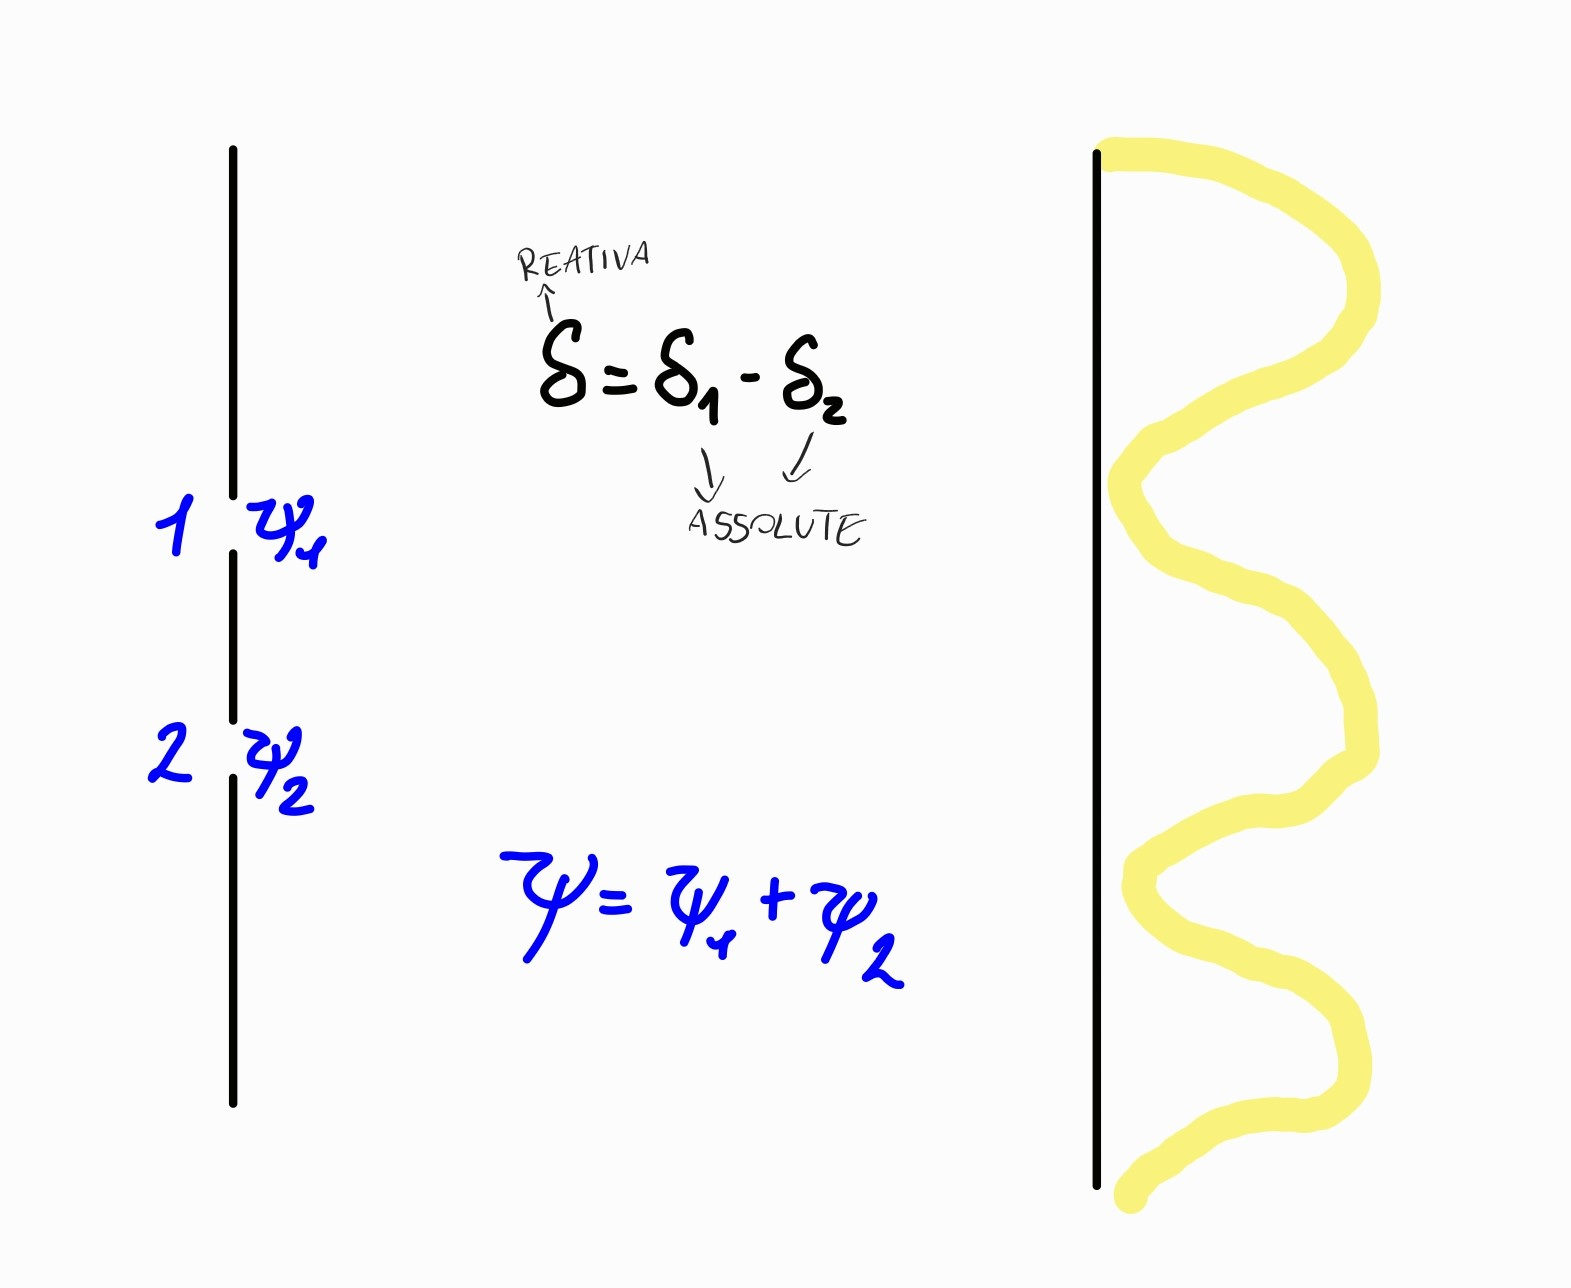
\includegraphics[width=0.31\textwidth]{Immagini/Doppia_fenditura.jpg}
    \caption{Esperimento della doppia fenditura.}
    \label{fig:fenditura}
\end{figure}
Quindi non è possibile misurare $\delta_1$ o $\delta_2$, ma solamente $\delta=\delta_1-\delta_2$. Inoltre, applicando delle trasformazioni del tipo $\delta_1\xrightarrow{}\delta_1+\alpha$ e $\delta_2\xrightarrow{}\delta_2+\alpha$ (con $\alpha$ una costante), la fase relativa $\delta$ rimane invariata. Trasformazioni di questo tipo sono dette \textit{trasformazioni globali di fase}\footnote{Il termine globale significa che la ridefinizione della fase è la stessa per tutti i punti dello spaziotempo.}, sotto queste trasformazioni la funzione d'onda varia in modo semplice:
\begin{equation}
    \psi\xrightarrow{}e^{i\alpha}\psi
\end{equation}
e la meccanica quantistica è invariante per questo tipo di trasformazioni. Infatti, se consideriamo il valor medio di un'osservabile generico , questo è indipendente dalla fase scelta:
\begin{equation}
    <\hat{O}>=\int\psi^*\hat{O}\psi d^3x
\end{equation}
Il gruppo che formano queste trasformazioni è detto $U(1)$. Possiamo, quindi, dire che la meccanica quantistica ha una simmetria di tipo $U(1)$ globale.

Ora, ci chiediamo cosa succede per trasformazioni $U(1)$ locali\footnote{Il termine locale indica semplicemente che la ridefinizione di fase varia, potenzialmente, punto per punto.}, ovvero trasformazioni del tipo:
\begin{equation}
    \psi\xrightarrow{}e^{i\alpha(t,\Vec{x})}\psi
\end{equation}
questo tipo di trasformazioni non sono simmetrie per nessuna teoria che descrive particelle libere, per esempio la \eqref{eq:eq_sch_part_lib}. Tuttavia, noi vogliamo forzare questo tipo di simmetria, per farlo è necessario modificare le teorie. Se, per esempio, prendiamo l'equazione \eqref{eq:eq_sch_part_car}, che descrive una particella carica sottoposta ad un campo elettromagnetico, abbiamo visto, nella sottosezione precedente, che vale una simmetria $U(1)$ locale, poiché $\chi(t,\Vec{x})$ dipende dalle coordinate spaziotemporali. Eppure, il costo da pagare è non banale. Infatti, affinché la teoria avesse la simmetria di gauge\footnote{Che è a tutti gli effetti una trasformazione $U(1)$ locale.}, è stato necessario introdurre nella teoria i campi $\Vec{A}$ e $\Phi$ e le rispettive trasformazioni di gauge. Quindi, possiamo dire, che le interazioni vengono dedotte imponendo delle simmetrie locali. L'idea è, dunque, di introdurre un'interazione a partire da una richiesta di simmetria locale. Tale procedura è quella usata per derivare tutte le interazioni fondamentali, ad esclusione di quella gravitazionale.

Possiamo riassumere quanto detto con il seguente enunciato del \textit{principio di gauge}: sia data una teoria che ha una simmetria globale rispetto ad un gruppo di Lie con $n$ generatori, si vuole imporre che la simmetria diventi locale, per farlo è necessario aggiungere alla teoria $n$ nuovi campi, i quali rappresentano nuove interazioni.

Ora applichiamolo ad un esempio di teoria di campo visto in precedenza.

Considerando un campo $\phi$ scalare complesso, possiamo definire la lagrangiana di Klein-Gordon:
\begin{equation}
  \mathcal{L}_{KG}=\partial_\mu\phi^*\partial^\mu\phi-\mu^2\phi^*\phi
\end{equation}
Otteniamo le equazioni di Eulero-Lagrange:
\begin{equation}
  (\Box+\mu^2)\phi^*=0 \qquad (\Box+\mu^2)\phi=0 
\end{equation}
tali equazioni lineari descrivono due particelle diverse di spin pari a zero e con la stessa massa, infatti questa formulazione viene usata per descrivere una particella e l'antiparticella corrispondente.

Sappiamo che, oltre alla simmetria per il gruppo di Poincaré, questa lagrangiana ha anche una simmetria interna per le trasformazioni:
\begin{equation}
\begin{gathered}
    \phi(x^\mu)\xrightarrow[\text{}]{\text{}}e^{i\alpha}\phi(x^\mu)\\
    \phi^*(x^\mu)\xrightarrow[\text{}]{\text{}}e^{-i\alpha}\phi^*(x^\mu)\\
    \partial_\mu \phi(x^\mu)\xrightarrow[\text{}]{\text{}}e^{i\alpha}\partial_\mu\phi(x^\mu)\\
   \partial_\mu \phi^*(x^\mu)\xrightarrow[\text{}]{\text{}}e^{-i\alpha}\partial_\mu\phi^*(x^\mu)\\
\end{gathered}
\end{equation}
ove $\alpha$ è una costante, tale simmetria porta con se la conservazione della carica. La simmetria in questione, per quanto detto precedentemente, è del tipo $U(1)$ globale. Le equazioni di Klein-Gordon descrivono particelle libere, tuttavia fisicamente viene da domandarsi per quale ragione particelle cariche non interagiscano. Per far emergere l'interazione dobbiamo usare il principio di gauge.

Quindi imponiamo che la simmetria da globale diventi locale, le trasformazioni per cui deve esserci simmetria, allora sono del tipo:
\begin{equation}
\begin{gathered}
    \phi(x^\mu)\xrightarrow[\text{}]{\text{}} \phi'(x^\mu)=e^{i\alpha(x^\mu)}\phi(x^\mu)\\
    \phi^*(x^\mu)\xrightarrow[\text{}]{\text{}}\phi'^*(x^\mu)=e^{-i\alpha(x^\mu)}\phi^*(x^\mu)\\
    \partial_\mu \phi(x^\mu)\xrightarrow[\text{}]{\text{}}\partial_\mu \phi'(x^\mu)=\partial_\mu[e^{i\alpha(x^\mu)}\phi(x^\mu)]\\
   \partial_\mu \phi^*(x^\mu)\xrightarrow[\text{}]{\text{}} \partial_\mu \phi'^*(x^\mu)=\partial_\mu[e^{-i\alpha(x^\mu)}\phi^*(x^\mu)]\\
\end{gathered}
\end{equation}
sviluppando i termini di derivata, otteniamo:
\begin{equation}
\begin{gathered}
    \partial_\mu \phi'(x^\mu)=\partial_\mu[e^{i\alpha(x^\mu)}\phi(x^\mu)]=e^{i\alpha(x^\mu)}[\partial_\mu\phi(x^\mu)]+i[\partial_\mu\alpha(x^\mu)]e^{i\alpha(x^\mu)}\phi(x^\mu)\\
  \partial_\mu \phi'^*(x^\mu)=\partial_\mu[e^{-i\alpha(x^\mu)}\phi^*(x^\mu)]=e^{-i\alpha(x^\mu)}[\partial_\mu\phi^*(x^\mu)]-i[\partial_\mu\alpha(x^\mu)]e^{-i\alpha(x^\mu)}\phi^*(x^\mu)\\
\end{gathered}
\end{equation}
il termine cinetico è dato dal prodotto tra i due:
\begin{equation}
\begin{aligned}
      \partial_\mu \phi'\partial^\mu \phi'^*&= \partial_\mu \phi\partial^\mu \phi^*-i\phi^*(\partial_\mu\phi)\partial^\mu\alpha+i\phi(\partial^\mu\phi^*)\partial_\mu\alpha+\partial_\mu\alpha\partial^\mu\alpha\phi^*\phi\\
      &=\partial_\mu \phi\partial^\mu \phi^*+i(\phi\partial_\mu\phi^*-\phi^*\partial_\mu\phi)\partial^\mu\alpha+\partial_\mu\alpha\partial^\mu\alpha\phi^*\phi
\end{aligned}
\end{equation}
il termine di massa è dato da:
\begin{equation}
\mu^2\phi'^*\phi'=\mu^2\phi^*\phi
\end{equation}

Concludiamo che a seguito di una trasformazione $U(1)$ locale, il termine di massa della lagrangiana va in se stesso, al contrario del termine cinetico, otteniamo, quindi, che la trasformazione proposta non è una simmetria per la lagrangiana di Klein-Gordon. Per forzare la simmetria modifichiamo la teoria, e dunque la lagrangiana, sostituendo la quadridivergenza con la derivata di gauge covariante\footnote{Questa, per definizione, deve trasformarsi come il campo, si usa dire che deve trasformasi vettorialmente.}. Le trasformazioni locali diventano\footnote{A queste trasformazioni abbiamo aggiunto un termine $e$ all'esponenziale, questo ci serve più avanti, comunque essendo una costante siamo liberi di farlo senza intaccare quanto detto sulle simmetrie $U(1)$ locali.}, quindi:
\begin{equation}
\begin{gathered}
    \phi(x^\mu)\xrightarrow[\text{}]{\text{}} \phi'(x^\mu)=e^{ie\alpha(x^\mu)}\phi(x^\mu)\\
    \phi^*(x^\mu)\xrightarrow[\text{}]{\text{}}\phi'^*(x^\mu)=e^{-ie\alpha(x^\mu)}\phi^*(x^\mu)\\
    D_\mu \phi(x^\mu)\xrightarrow[\text{}]{\text{}}D'_\mu \phi'(x^\mu)=e^{ie\alpha(x^\mu)}D_\mu\phi(x^\mu)\\
   D^*_\mu \phi^*(x^\mu)\xrightarrow[\text{}]{\text{}} D'^*_\mu \phi'^*(x^\mu)=e^{-ie\alpha(x^\mu)}D^*_\mu\phi^*(x^\mu)\\
\end{gathered}
\end{equation}
ove, ricordiamo, la derivata di gauge è definita come $D_\mu=\partial_\mu+iqA_\mu$, con $A_\mu$ detto campo di gauge\footnote{Il numero di campi di gauge da introdurre, affinché si possa imporre una simmetria, deve essere pari al numero di generatori del gruppo di cui si richiede la simmetria. In questo caso $U(1)$ ha un solo generatore e quindi il campo introdotto è uno solo; se la simmetria fosse stata imposta per il gruppo $SU(2)$, allora i campi da introdurre sarebbero stati tre, poiché i generatori del gruppo sono tre.}. D'ora in poi considereremo $q=-e$, quindi la derivata di gauge sarà $D_\mu=\partial_\mu-ieA_\mu$. Studiamo i nuovi termini di derivazione:
\begin{equation}
\begin{gathered}
    D'_\mu \phi'=[\partial_\mu-ieA'_\mu](e^{ie\alpha}\phi)=e^{ie\alpha}D_\mu\phi=e^{ie\alpha}[\partial_\mu-ieA_\mu]\phi\\
  e^{ie\alpha}(\partial_\mu\phi+ie\phi\partial_\mu\alpha-ieA'_\mu\phi)=e^{ie\alpha}[\partial_\mu\phi-ieA_\mu\phi]\\
  +ie\phi\partial_\mu\alpha-ieA'_\mu\phi=-ieA_\mu\phi\\
  A'_\mu=A_\mu+\partial_\mu\alpha
\end{gathered}
\end{equation}
Imponendo come si deve trasformare la derivata di gauge, abbiamo trovato come si trasforma il campo di gauge ad essa associato, lo stesso procedimento lo si può fare anche con il campo complesso coniugato $\phi^*$.

Alla luce di questo, scrivere una lagrangiana che abbia una simmetria $U(1)$ locale, diventa banale:
\begin{equation}
  \mathcal{L}=D_\mu\phi(D^\mu\phi)^*-\mu^2\phi^*\phi=(\partial_\mu-ieA_\mu)\phi(\partial^\mu+ieA^\mu)\phi^*-\mu^2\phi^*\phi
\end{equation}
tuttavia neanche questa teoria è completa, perché manca il termine cinetico di $A_\mu$, ossia $\partial_\nu A_\mu$, il quale ne descrive la dinamica. Quindi dobbiamo aggiungere un termine alla lagrangiana, ovviamente tale termine dovrà rispettare tutti i requisiti necessari al fine che la lagrangiana soddisfi tutte le proprietà richieste (gauge invarianza e simmetria gruppo di Poincaré).
\begin{equation}
  \mathcal{L}_{QED}=(\partial_\mu-ieA_\mu)\phi(\partial^\mu+ieA^\mu)\phi^*-\mu^2\phi^*\phi-\dfrac{1}{16\pi}F_{\mu\nu}F^{\mu\nu}
\end{equation}
questa è detta \textit{lagrangiana dell'elettrodinamica scalare}.

Sviluppando i termini si ottiene:
\begin{equation}
\begin{aligned}
     \mathcal{L}_{QED}&=\partial_\mu\phi\partial^\mu\phi^*-\mu^2\phi^*\phi+ieA^\mu(\phi^*\partial_\mu\phi-\phi\partial_\mu\phi^*)+e^2A_\mu A^\mu\phi^*\phi-\dfrac{1}{16\pi}F_{\mu\nu}F^{\mu\nu}\\
     &=\mathcal{L}_{KG}+\mathcal{L}_{INT}+\mathcal{L}_{M}
\end{aligned}
\end{equation}
Possiamo notare che i primi due termini sono la lagrangiana di Klein-Gordon (per particelle libere), i termini terzo, quarto e quinto sono la lagrangiana che descrive le interazioni (poiché hanno dipendenze dai campi superiori a due), infine il sesto è la lagrangiana  di Maxwell per il campo di gauge. 

Ci rimane da calcolare le equazioni di Eulero-Lagrange, per i tre campi indipendenti $\phi$, $\phi^*$ e $A_\nu$. Partiamo da $\phi^*$:
\begin{equation}
\begin{gathered}
      \partial_\mu\dfrac{\partial \mathcal{L}_{QED}}{\partial(\partial_\mu \phi^*)}=\dfrac{\partial\mathcal{L}_{QED}}{\partial \phi^*} \\
      \partial_\mu(\partial^\mu\phi-ieA^\mu\phi)=-\mu^2\phi+ieA^\mu\partial_\mu\phi+e^2A_\mu A^\mu\phi\\
      \Box\phi+\mu^2\phi=ie\partial_\mu(A^\mu\phi)+ieA^\mu\partial_\mu\phi+e^2A_\mu A^\mu\phi
\end{gathered}
\end{equation}
in maniera del tutto analoga, l'equazione per $\phi$ si determina semplicemente sostituendo con il complesso coniugato:
\begin{equation}
      \Box\phi^*+\mu^2\phi^*=ie\partial_\mu(A^\mu\phi^*)+ieA^\mu\partial_\mu\phi^*+e^2A_\mu A^\mu\phi^*
\end{equation}
Infine, rimane solamente $A_\nu$:
\begin{equation}
\begin{gathered}
    \partial_\mu\dfrac{\partial \mathcal{L}_{QED}}{\partial(\partial_\mu A_\nu)}=\dfrac{\partial\mathcal{L}_{QED}}{\partial A_\nu}\\
    \partial\left(-\dfrac{F^{\mu\nu}}{4\pi}\right)=ie(\phi^*\partial^\nu\phi-\phi\partial^\nu\phi^*)+2A^\nu\phi\phi^*\\
    \partial_\mu F^{\mu\nu}=4\pi[ie(\phi\partial^\nu\phi^*-\phi^*\partial^\nu\phi)-2A^\nu\phi\phi^*]
\end{gathered}
\end{equation}
Quindi è un sistema di tre campi accoppiati tra loro, la cui dinamica è descritta da queste tre equazioni.

\subsection{Rottura spontanea di simmetria}
Lo studio effettuato nella sezione precedente è valido solo per interazioni i cui mediatori sono campi non massivi. Infatti, per rendere il campo massivo dovremmo aggiungere nella lagrangiana un termine di massa di Proca $(m^2A_\mu A^\mu)$, però come abbiamo già visto questo termine rompe la gauge invarianza della lagrangiana.

\`E possibile aggirare lostacolo mediante la così detta \textit{rottura spontanea di simmetria}. Questo concetto, prima che venisse usato nella teoria dei campi, era già noto nell'ambito della fisica della materia condensata. Un esempio ci è dato dal ferromagnetismo. In un ferromagnete ci sono vari domini di spin, sappiamo che sopra la temperatura di Curie i domini sono orientati isotropicamente, mentre sotto la temperatura di Curie gli spin si allineano dando origine ad una magnetizzazione netta.
\begin{figure}[H]
    \centering
    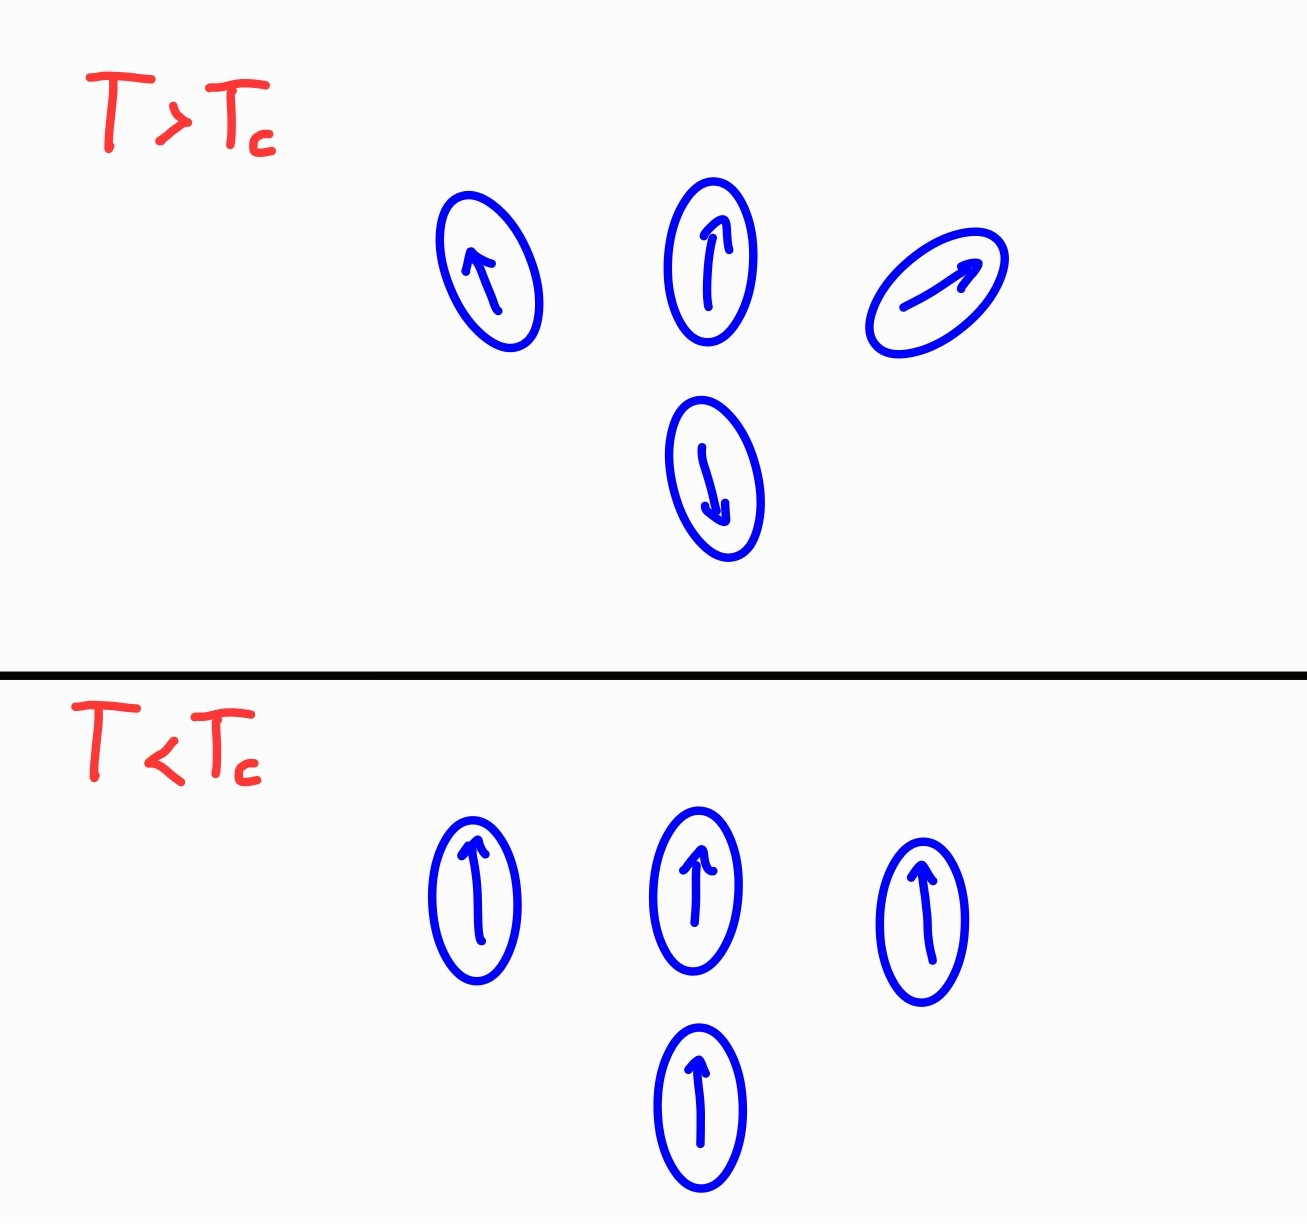
\includegraphics[width=0.31\textwidth]{Immagini/Spin.jpg}
    \caption{Spin di un ferromganete.}
    \label{fig:ferromagnete}
\end{figure}
L'Hamiltoniana associata è del tipo $H=-\sum_{i\neq j}\mu_{ij}\Vec{s}_i\cdot\Vec{s}_j$, questa risulta essere invariante per rotazioni. Tuttavia, nel caso $T<T_C$ il sistema o, meglio, lo stato fondamentale del sistema rompe l'invarianza per rotazioni.

Generalizzando il concetto, possiamo dire che: data una teoria con una certa simmetria, se lo stato fondamentale non rispetta tale simmetria, allora si parla di rottura spontanea di simmetria.

Analizziamo, ora, un esempio di teoria di campo visto in precedenza.

Consideriamo un campo scalare reale con una lagrangiana del tipo:
\begin{equation}\phantomsection\label{eq:lag}
  \mathcal{L}(\phi,\partial_\mu\phi)=\partial_\mu\phi\partial^\mu\phi-V(\phi)
\end{equation}
dall'equazione di Eulero-Lagrange
\begin{equation}
    \partial_\mu\dfrac{\partial \mathcal{L}}{\partial(\partial_\mu\phi)}-\dfrac{\partial\mathcal{L}}{\partial \phi}=0
\end{equation}
otteniamo l'equazione del moto:
\begin{equation}
   \Box \phi+\dfrac{dV}{d\phi}=0
\end{equation}
In generale, per teorie di questo tipo abbiamo che il momento coniugato è
\begin{equation}
    \mathcal{P}=\dfrac{\partial\mathcal{L}}{\partial \Dot{\phi}}=\Dot{\phi} \quad \text{ove }\quad\dot{\phi}=\dfrac{\partial \phi}{\partial t}
\end{equation}
Quindi possiamo definire una Hamiltoniana:
\begin{equation}
    H=\int d^3x\mathcal{H}
\end{equation}
ove la densità di Hamiltoniana è definita come:
\begin{equation}
    \mathcal{H}=\mathcal{P}\dot{\phi}-\mathcal{L}=\dfrac{\dot{\phi}^2}{2}+\left(\Vec{\nabla}\phi\right)^2+V(\phi)
\end{equation}
Ora, ci chiediamo quale sia la configurazione di campo che minimizzi l'Hamiltoniana. Osservando la forma analitica vediamo che l'Hamiltoniana sarà minima per $\phi$ constante (così che i primi due termini siano nulli) e il $\phi$ che minimizza il potenziale $V(\phi)$.

 Consideriamo il seguente potenziale
 \begin{equation}\phantomsection\label{eq:pot_1}
    V(\phi)=\dfrac{1}{2}m^2\phi^2+\dfrac{1}{4}\lambda\phi^4
\end{equation}
ove richiediamo che $\lambda>0$, altrimenti $ V(\phi)\xrightarrow{\phi\xrightarrow{}\infty}-\infty$, per cui non avremo alcun punto di minimo globale sul quale fissare lo stato fondamentale. Studiando il potenziale troviamo che ha forma:
\begin{figure}[H]
    \centering
    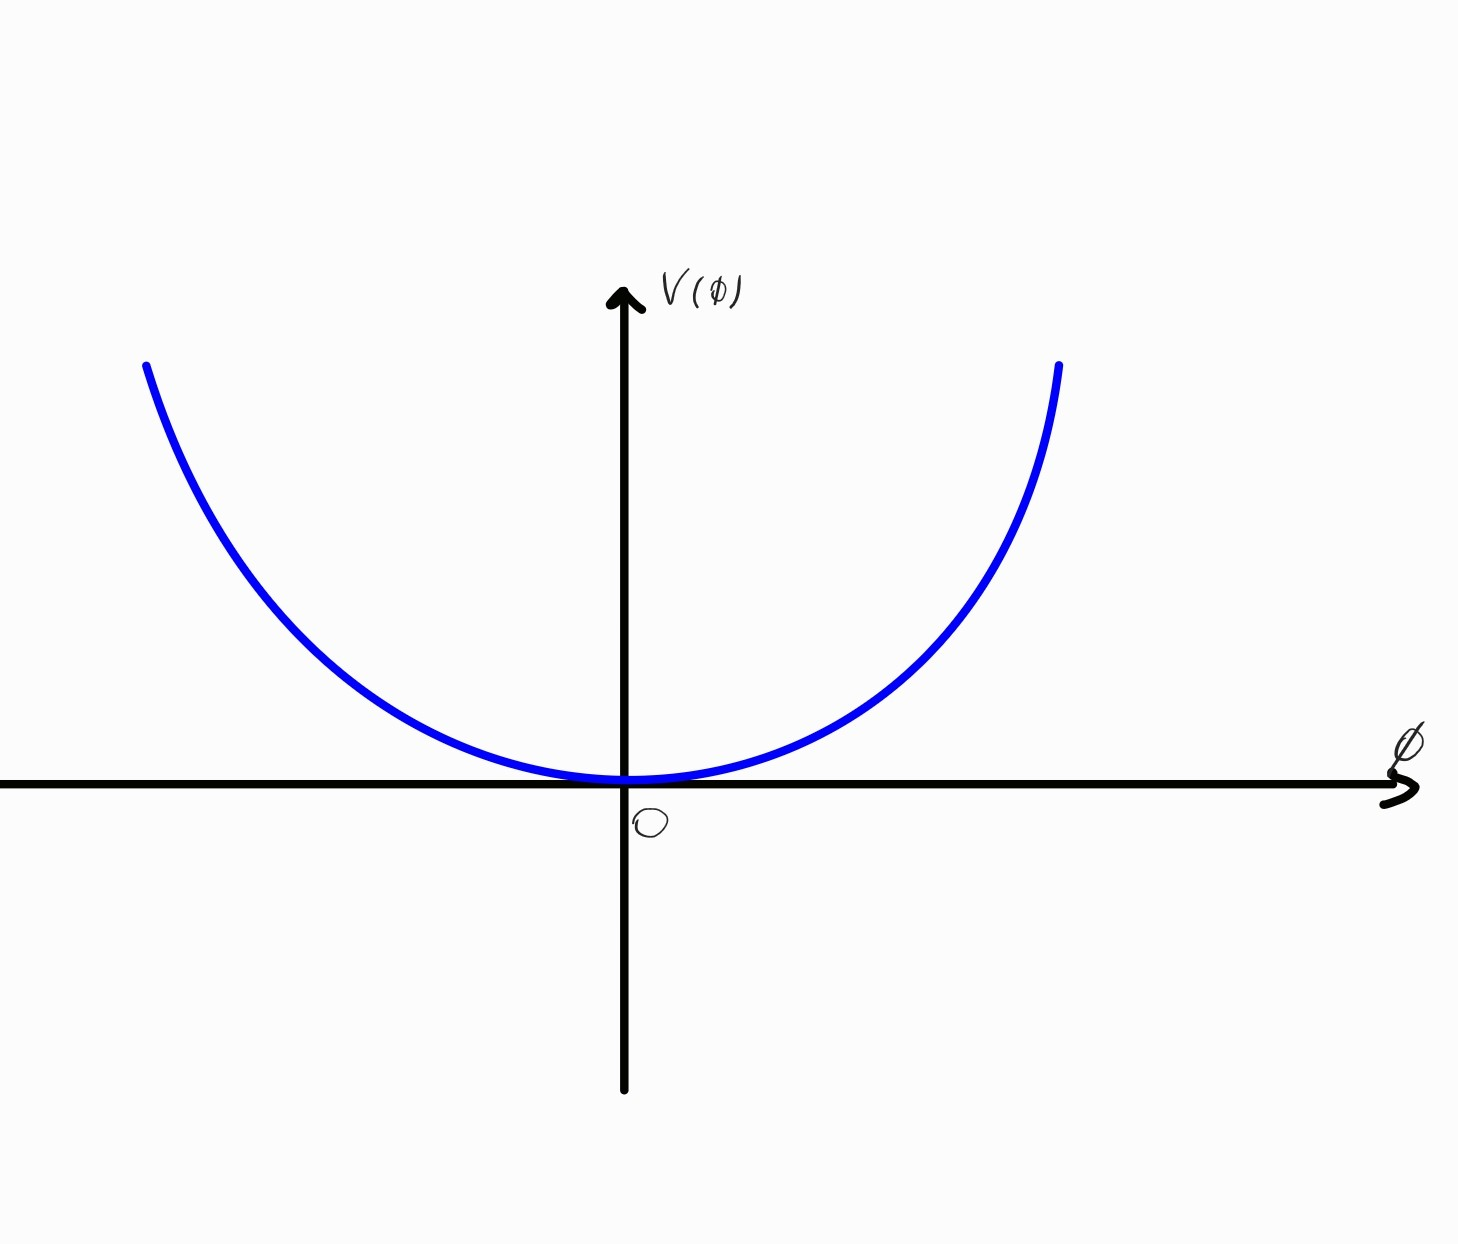
\includegraphics[width=0.31\textwidth]{Immagini/Pot1.jpg}
    \caption{Potenziale $ V(\phi)=\dfrac{1}{2}m^2\phi^2+\dfrac{1}{4}\lambda\phi^4$.}
    \label{fig:pot1}
\end{figure}
per cui fissiamo lo stato fondamentale nel punto $\phi=0$.

Osserviamo che la lagrangiana \eqref{eq:lag} con potenziale \eqref{eq:pot_1} ha una simmetria per la trasformazione discreta di parità $\phi\xrightarrow{}-\phi$, inoltre notiamo che a seguito di una tale trasformazione lo stato fondamentale rimane invariato; in tal caso si parla di \textit{simmetria ordinaria}.

Dall'equazione di Eulero-Lagrange otteniamo:
\begin{equation}
    (\Box+m^2)\phi=-\lambda\phi^3
\end{equation}
che descrive particelle massive di spin nullo, il temine cubico rappresenta l'autointerazione del campo.

 Consideriamo un altro potenziale
 \begin{equation}\phantomsection\label{eq:pot_2}
    V(\phi)=-\dfrac{1}{2}\mu^2\phi^2+\dfrac{1}{4}\lambda\phi^4
\end{equation}
sempre con $\lambda>0$ e c'è la simmetria per $\phi\xrightarrow{}-\phi$. Possiamo, inoltre, osservare che, apparentemente, la massa sia immaginaria, d'altronde l'equazione di campo assume la forma:
\begin{equation}
    (\Box-\mu^2)\phi=-\lambda\phi^3
\end{equation}

Derivando il potenziale troviamo:
 \begin{equation}
    \dfrac{\partial V(\phi)}{\partial \phi}=-\mu^2\phi+\lambda\phi^3
\end{equation}
da cui i punti critici sono per:
\begin{equation}
   \phi=0 \quad\land\quad\phi=\pm\sqrt{\dfrac{\mu^2}{\lambda}}=\pm v
\end{equation}
graficandola:
\begin{figure}[H]
    \centering
    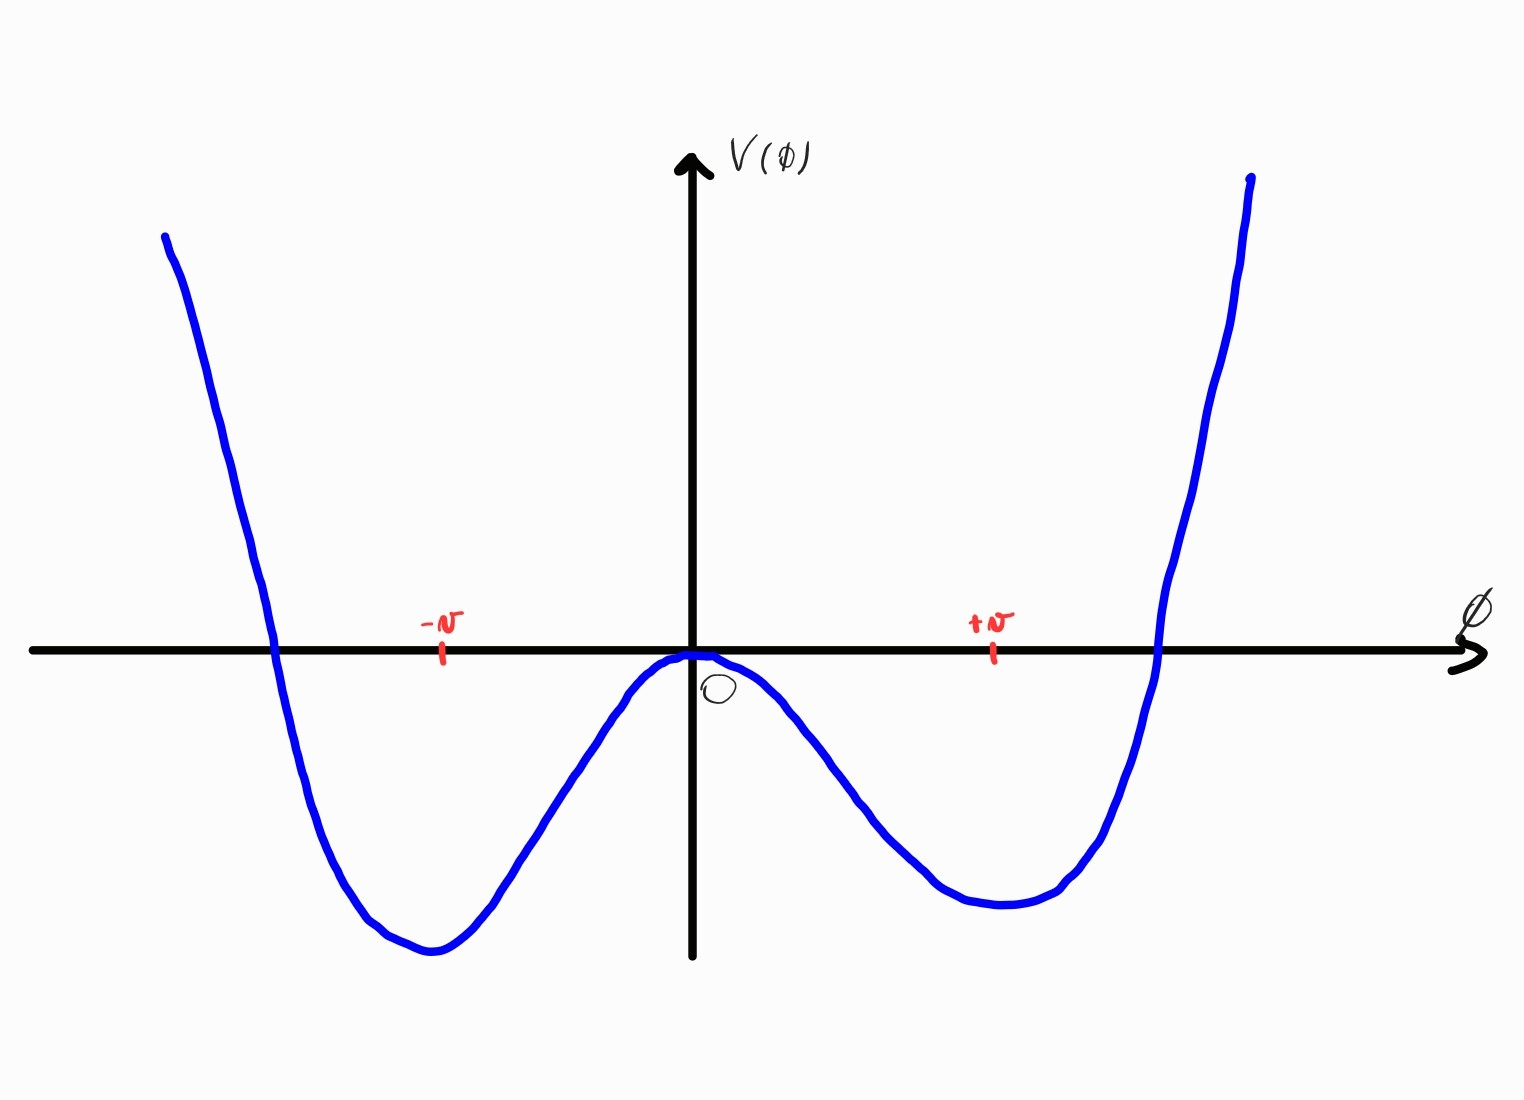
\includegraphics[width=0.31\textwidth]{Immagini/Pot2.jpg}
    \caption{Potenziale $ V(\phi)=-\dfrac{1}{2}\mu^2\phi^2+\dfrac{1}{4}\lambda\phi^4$.}
    \label{fig:pot2}
\end{figure}
ci accorgiamo che il punto $\phi=0$ è di massimo locale e dunque, essendo instabile, non può essere lo stato fondamentale. Scegliamo come stato fondamentale $\phi=v$, ci accorgiamo che applicando una trasformazione di parità lo stato fondamentale non rimane lo stesso, ecco che si verifica la rottura spontanea di simmetria.
Inoltre, la questione della massa immaginaria si risolve autonomamente, infatti per dire che la massa era immaginaria bisognava implicitamente assumere come stato fondamentale $\phi=0$, ma questo non lo è.

 Vogliamo studiare le fluttuazioni del campo rispetto allo stato fondamentale, per farlo definiamo un nuovo campo:
 \begin{equation}
     \phi'(x)=\phi-v
 \end{equation}
questo mi parametrizza le oscillazioni attorno allo stato fondamentale. Riscriviamo la lagrangiana in termini del nuovo campo:
\begin{equation}\phantomsection\label{eq:lag_phi'}
  \mathcal{L}=\partial_\mu\phi'\partial^\mu\phi'-V(\phi')
\end{equation}
il potenziale sarà:
\begin{equation}
\begin{aligned}
      V(\phi')&=-\dfrac{1}{2}\mu^2(\phi'+v)^2+\dfrac{1}{4}\lambda(\phi'+v)^4\\
      &=-\dfrac{\mu^2}{2}(\phi'^2+2\phi' v+v^2)+\dfrac{\lambda}{4}(\phi'^4+4\phi'^3v+6\phi'^2v^2+4\phi' v^3+v^4)
\end{aligned}
\end{equation}
 studiamo ogni termine in funzione dell'ordine di $\phi'$:
 \begin{equation}
\begin{aligned}
 &\phi'^0:      \quad  -\dfrac{\mu^2}{2}v^2+\dfrac{\lambda}{4} v^4\\
  &\phi':      \quad   -\mu^2v+\lambda v^3=   v(-\mu^2+\lambda v^2)=0                                        \\
 & \phi'^2:     \quad -\dfrac{\mu^2}{2}+\dfrac{3}{2}\lambda v^2=\mu^2                                              \\
 & \phi'^3:  \quad             \lambda v                                             \\
 & \phi'^4:\quad       \dfrac{\lambda}{4}
\end{aligned}\footnote{Come avevamo già capito il termine di massa non ha massa immaginaria una volta fissato il giusto stato fondamentale.}
\end{equation}
Il potenziale assume, quindi, la forma:
\begin{equation}\phantomsection\label{eq:pot_phi'}
      V(\phi')=-\mu^2 \phi'^2+\mu^2\left[\dfrac{1}{v}\phi'^3+\dfrac{1}{4v^2}\phi'^4-\dfrac{\mu^2}{4\lambda}\right]
\end{equation}
l'equazione di Eulero-Lagrange è:
\begin{equation}
    (\Box+2\mu^2)\phi'=-\dfrac{3\mu^2}{v}\phi'^2-\dfrac{\mu^2}{v^2}\phi'^4
\end{equation}
 se chiamiamo $m^2=2\mu^2\xrightarrow{}m=\sqrt{2}\mu$, abbiamo trovato che la massa è reale.

 Anche per la lagrangiana \eqref{eq:lag_phi'} con il potenziale \eqref{eq:pot_phi'} vale la simmetria per la trasformazione di parità $\phi\xrightarrow{}-\phi$, anche se non è manifesta.



Nei due casi appena esaminati avevamo che la simmetria era di tipologia discreta, ora vogliamo esaminare casi in cui la simmetria sia continua.




 Per farlo, consideriamo due campi scalari reali $\phi_1$ e $\phi_2$, con una lagrangiana del tipo:
\begin{equation}
  \mathcal{L}=\dfrac{1}{2}(\partial_\mu\phi_1\partial^\mu\phi_1+\partial_\mu\phi_2\partial^\mu\phi_2)-V(\phi_1^2+\phi_2^2)
\end{equation}
questa lagrangiana ha una simmetria continua di tipo $SO(2)$:

\begin{equation}
   \begin{pmatrix}
 \phi_1' \\
\phi_2'\\
\end{pmatrix}=\begin{pmatrix}
 \cos{\theta}&\sin{\theta}\\
-\sin{\theta} &\cos{\theta}\\
\end{pmatrix} \begin{pmatrix}
 \phi_1 \\
\phi_2\\
\end{pmatrix}
\end{equation}
Consideriamo un potenziale del tipo
\begin{equation}
    V(\phi_1^2+\phi_2^2)=\dfrac{m^2}{2}(\phi_1^2+\phi_2^2)+\dfrac{\lambda}{4}(\phi_1^2+\phi_2^2)^2
\end{equation}
determiniamo lo stato fondamentale, per farlo calcoliamo le derivate del potenziale:
\begin{equation}
    \begin{cases}
        \dfrac{\partial V}{\partial\phi_1}=m^2\phi_1+\lambda\phi_1(\phi_1^2+\phi_2^2)=0\\
        \\
        \dfrac{\partial V}{\partial\phi_2}=m^2\phi_2+\lambda\phi_2(\phi_1^2+\phi_2^2)=0
    \end{cases}
\end{equation}
risolvendo il sistema troviamo che la soluzione al sistema è $\phi_1=\phi_2=0$, questo è il nostro stato fondamentale.
La rappresentazione del potenziale è: 
\begin{figure}[H]
    \centering
    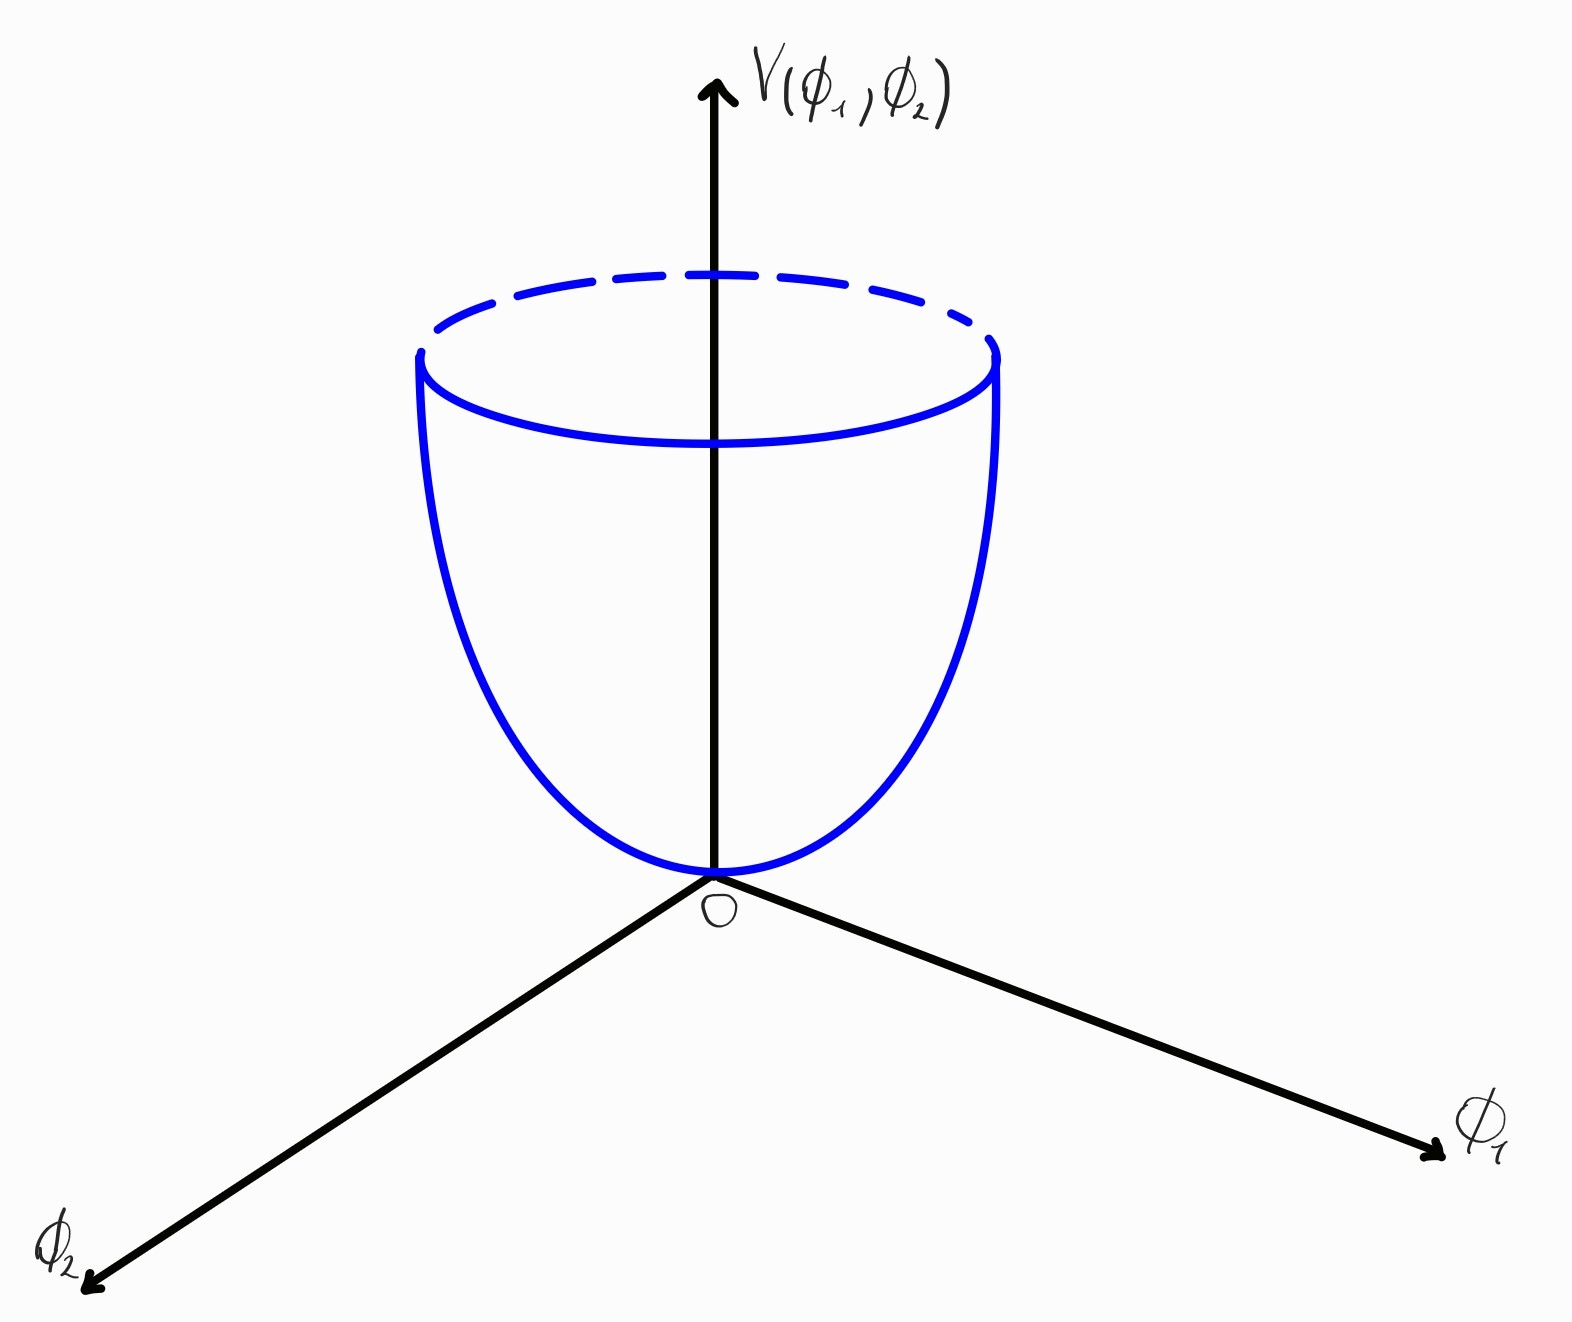
\includegraphics[width=0.31\textwidth]{Immagini/Pot3.jpg}
    \caption{Potenziale $ V(\phi_1^2+\phi_2^2)=\dfrac{m^2}{2}(\phi_1^2+\phi_2^2)+\dfrac{\lambda}{4}(\phi_1^2+\phi_2^2)^2$.}
    \label{fig:pot3}
\end{figure}
Per una rotazione nel piano dei campi lo stato fondamentale rimane fisso, quindi abbiamo una simmetria ordinaria.



Consideriamo un altro esempio, sempre a partire da due campi scalari reali $\phi_1$ e $\phi_2$, con un potenziale del tipo
\begin{equation}
    V(\phi_1^2+\phi_2^2)=-\dfrac{\mu^2}{2}(\phi_1^2+\phi_2^2)+\dfrac{\lambda}{4}(\phi_1^2+\phi_2^2)^2
\end{equation}
anche qui sembra esserci un massa immaginaria, tuttavia ormai abbiamo compreso non essere sempre così semplice.

Determiniamo lo stato fondamentale, le derivate del potenziale sono:
\begin{equation}
    \begin{cases}
        \dfrac{\partial V}{\partial\phi_1}=-\mu^2\phi_1+\lambda\phi_1(\phi_1^2+\phi_2^2)=0\\
        \\
        \dfrac{\partial V}{\partial\phi_2}=-\mu^2\phi_2+\lambda\phi_2(\phi_1^2+\phi_2^2)=0
    \end{cases}
\end{equation}
risolvendo il sistema troviamo che la soluzione si ha per $\phi_1=\phi_2=0$ e per $\phi_1^2+\phi_2^2=\dfrac{\mu^2}{\lambda}=v^2$, ove quest'ultima è una circonferenza.

La rappresentazione del potenziale è: 
\begin{figure}[H]
    \centering
    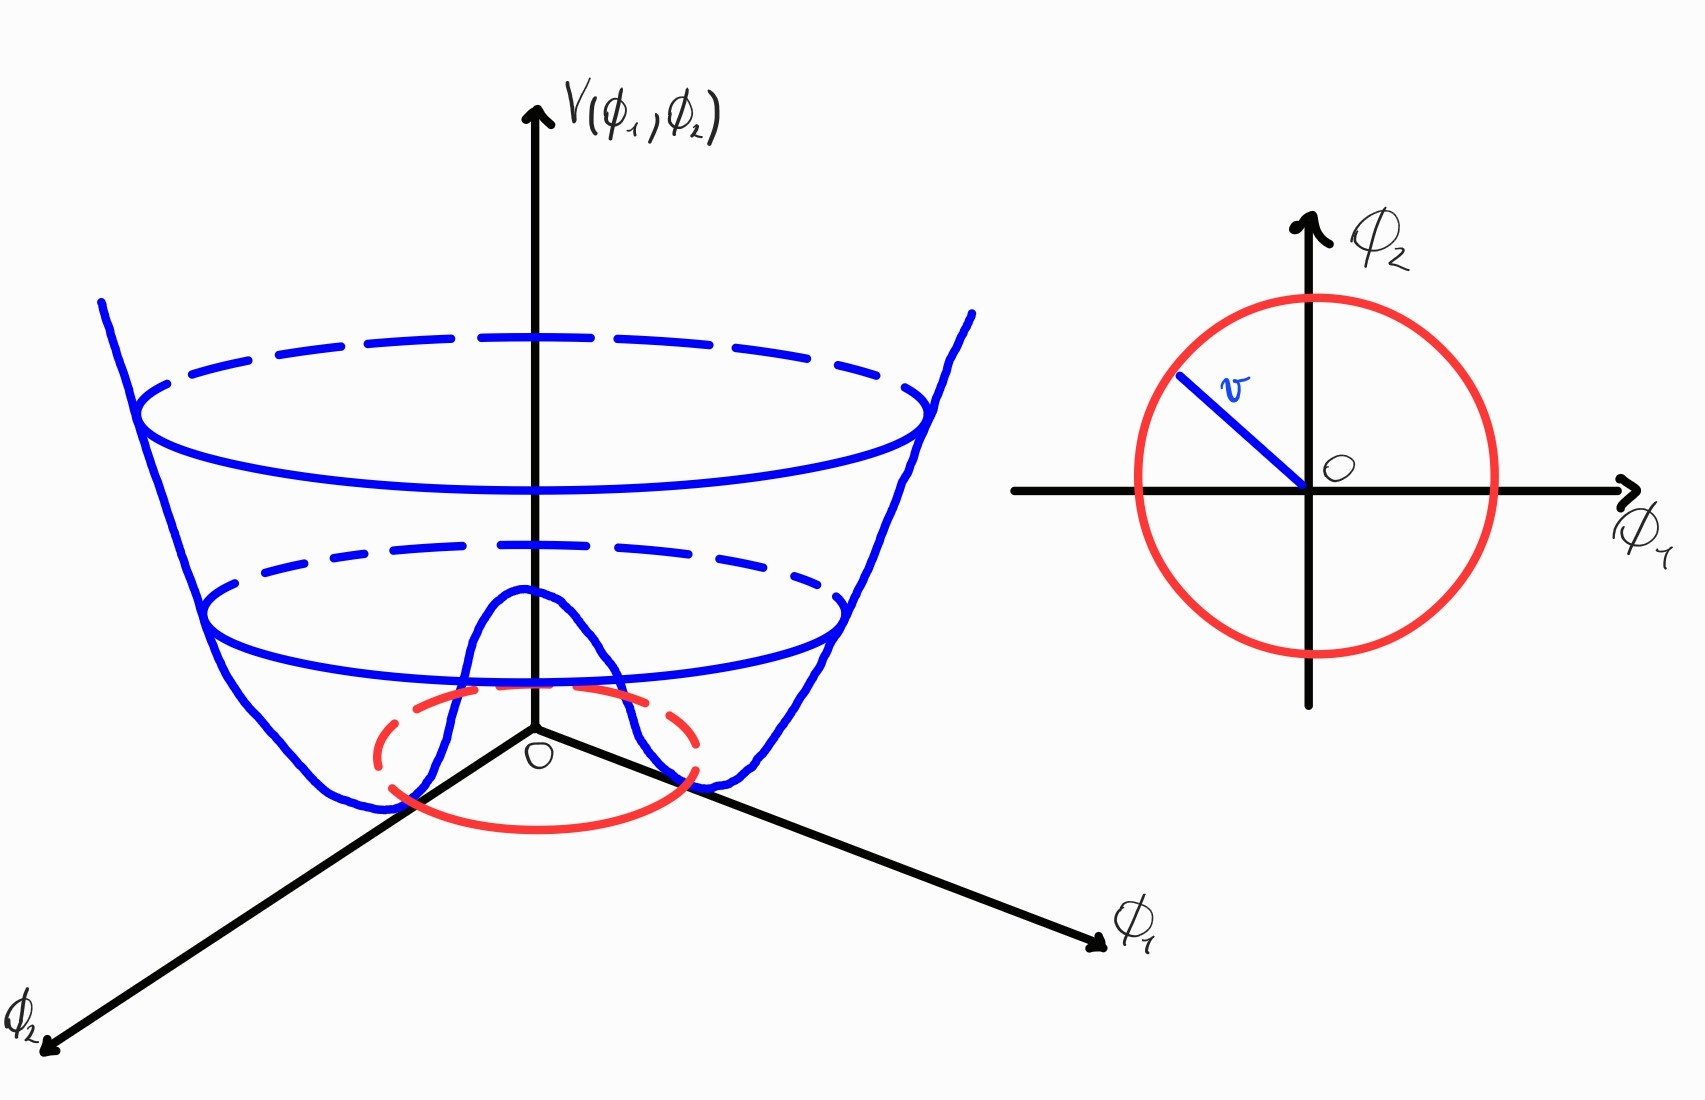
\includegraphics[width=0.31\textwidth]{Immagini/Pot4.jpg}
    \caption{Potenziale $  V(\phi_1^2+\phi_2^2)=-\dfrac{\mu^2}{2}(\phi_1^2+\phi_2^2)+\dfrac{\lambda}{4}(\phi_1^2+\phi_2^2)^2$.}
    \label{fig:pot4}
\end{figure}
Notiamo che il punto $\phi_1=\phi_2=0$ è un massimo e dunque non è lo stato fondamentale, al contrario dei punti corrispondenti alla circonferenza, possiamo, quindi, scegliere in maniera arbitraria un punto tra questi, per semplicità scegliamo $\phi_1=v$ e $\phi_2=0$.
Vogliamo capire che tipo di particelle rappresenta la teoria, per falo dobbiamo studiare le fluttuazioni del campo rispetto allo stato fondamentale, quindi definiamo
i nuovi campi:
\begin{equation}
 \eta=\phi'_1=\phi_1-v\qquad\xi=\phi'_2=\phi_2
\end{equation}
Per lo stato fondamentale non vi è la simmetria rispetto a $SO(2)$, quindi si ha la rottura spontanea di simmetria.

La lagrangiana riscritta in questi campi è:
\begin{equation}
  \mathcal{L}(\eta,\xi)=\dfrac{1}{2}\partial_\mu\eta\partial^\mu\eta+\dfrac{1}{2}\partial_\mu\xi\partial^\mu\xi-V(\eta,\xi)
\end{equation}
mentre il potenziale assume la forma
\begin{equation}
V(\eta,\xi)=-\dfrac{\mu^2}{2}[\eta^2+2\eta v+v^2+\xi^2]+\dfrac{\lambda}{4}[\eta^4+6\eta^2v^2+v^4+\xi^4+4\eta^3v+2\eta^2\xi^2+4\eta v^3+4v\eta\xi^2+2v^2\xi^2]
\end{equation}
 studiamo ogni termine in funzione dell'ordine di $\eta$ e $\xi$ (scriveremo solo i termini necessari a trarre le conclusioni):
 \begin{equation}
\begin{aligned}
 &\eta: \quad  -\mu^2 v+\lambda v^3=0\\  
 & \eta^2:     \quad -\dfrac{\mu^2}{2}+\dfrac{3}{2}\lambda v^2=\mu^2                                              \\
 & \xi:  \quad           0             \\
 & \xi^2:\quad      -\dfrac{\mu^2}{2}+\dfrac{1}{2}\lambda v^2=0\\
&\vdots
\end{aligned}
\end{equation}

Riscrivendo la lagrangiana abbiamo:
\begin{equation}
  \mathcal{L}(\eta,\xi)=\dfrac{1}{2}\partial_\mu\eta\partial^\mu\eta+\dfrac{1}{2}\partial_\mu\xi\partial^\mu\xi-\mu^2\eta^2+\cdots
\end{equation}
Quindi la teoria descrive una particella del campo $\eta$, che è massiva di massa $m=\sqrt{2}\mu$ reale, e una particella del campo $\xi$ non è massiva. La particella non massiva è chiamata \textit{bosone di Goldstone}.

Questo discende dal teorema di Goldstone il quale afferma che quando una simmetria continua viene spontaneamente rotta nello spettro di massa compaiono necessariamente delle particelle di massa nulla.



Ripercorriamo i punti fondamentali delle ultime pagine ed aggiungiamo alcune considerazioni.

La questione iniziale era che, considerando le teorie di gauge, a seguito del principio di gauge, queste comportavano l'introduzione dei campi di gauge non massivi, l'esempio che abbiamo visto era quello dell'elettrodinamica scalare. Tuttavia, noi vogliamo descrivere altri tipi di interazioni che hanno mediatori massivi, pur mantenendo le proprietà delle teorie di gauge. Il motivo per cui vogliamo mantenere queste proprietà risiede nel fatto che, quantisticamente, le teorie di gauge sono rinormalizzabili\footnote{Quindi è possibile attribuirgli un significato fisico.}. Con la rottura spontanea di simmetria, solo apparentemente, sembra di andare in direzione opposta al problema, poiché il teorema di Goldstone afferma l'esistenza di altri campi non massivi, cionondimeno avviene una sorta di miracolo quando si mette assieme la rottura spontanea di simmetria e le teorie di gauge. A livello di gradi di libertà, la differenza tra un campo vettoriale massivo e uno vettoriale non massimo è che il primo ha tre gradi di libertà (una direzione trasversale positiva, una direzione trasversale negativa e una longitudinale)\footnote{Lo abbiamo visto con la lagrangiana di Proca.}, il secondo solo due (una direzione trasversale positiva, una direzione trasversale negativa)\footnote{Lo abbiamo visto con la lagrangiana elettromagnetica}. Il miracolo che avviene sembra essere che, in qualche modo, il bosone di Goldstone venga fagocitato dal campo di gauge, donando, così, al campo di gauge massa e quindi tre possibili polarizzazioni. Nel processo di rottura della simmetria di gauge, la lagrangiana non perde tale simmetria proprio perché la rottura è spontanea; ciò che rompe la simmetria è la definizione dello stato fondamentale.





























